\documentclass[times, utf8, zavrsni, numeric]{fer}
\usepackage{booktabs}
\usepackage{graphicx}
\usepackage{subcaption}
\usepackage{gensymb}
\usepackage{indentfirst}
\usepackage{amssymb}
\usepackage{commath}
\usepackage{hyperref} 

\begin{document}

\thesisnumber{5187}
\title{Ekstrakcija tablica na skeniranim dokumentima}
\author{Kristijan Vulinović}

\maketitle

% Ispis stranice s napomenom o umetanju izvornika rada. Uklonite naredbu \izvornik ako želite izbaciti tu stranicu.
\izvornik

% Dodavanje zahvale ili prazne stranice. Ako ne želite dodati zahvalu, naredbu ostavite radi prazne stranice.
\zahvala{Zahvaljujem svima onima koji su odvojili dio svojeg vremena na ispunjavanje primjeraka tablica, kao i svima koji su pomogli prilikom prikupljanja istih.}

\tableofcontents

\chapter{Uvod}
U današnje vrijeme postoje izuzetno velike količine papirnatih dokumenata.
Samo u Sjedinjenim Američkim Državama nastaje više od milijarde novih papirnatih dokumenata svakog radnog dana. 
Mogućnost digitalizacije takvih dokumenata može biti od velike koristi prilikom pohrane, slanja ili pretraživanja istih. \cite{article:Skew-detection}
Digitalizaciju dokumenata možemo podijeliti u dva dijela: prepoznavanje teksta te prepoznavanje grafičkih objekata. \cite{conference:DetectionOfTableStructure} 
Za prepoznavanje teksta dostupan je velik broj alata koji omogućuju optičko prepoznavanje znakova (engl. \textit{optical character recognition}).
Prepoznavanje grafičkih objekata dokumenta mnogo je manje zastupljeno u odnosu na prepoznavanje teksta te je postalo popularnije tek u novije vrijeme. 
U to spada prepoznavanje linija, oblika, slika, simbola, tablica i raznih drugih objekata koji se mogu nalaziti na skeniranim dokumentima.
Najveći razvoj ovoga područja nastupio je zahvaljujući razvoju dubokih neuronskih mreža i sklopovlja koje omogućuje velike brzine izračuna koje prije nisu bile moguće.\\

Ovaj rad se fokusira isključivo na prepoznavanje tablica, što je prethodno već opisano u radovima poput \cite{conference:DetectionOfTableStructure} i \cite{conference:AutomaticTableDetectionInDocumentImages}. 
Taj postupak se dijeli na prepoznavanje položaja tablice u odnosu na ostatak dokumenta, prilikom čega je potrebno u dokumentu izdvojiti tablicu od ostatka teksta i ostalih grafičkih objekata, a što je opisano u radu \cite{article:Medium-IndependentTableDetection}.
Nakon što je tablica pronađena određuje se njezin izgled, odnosno broj redaka i stupaca, odnosno koordinate pojedine ćelije, a što je detaljnije opisano u nastavku rada. \\

Predstavljeno rješenje počinje od slike u sivim tonovima (engl. \textit{gray-scale}), koja se binarizira kako bi se dobila slika koja se sastoji od isključivo crne i bijele boje.
Dobivena crno-bijela slika koristi se u daljnjoj obradi te se provjerava je li slika rotirana, odnosno kut rotacije iste, nakon čega se slika po potrebi rotira kako bi tablica stajala okomito.
Ovako obrađena slika koristi se dalje za detekciju tablica, postupkom koji se temelji na prepoznavanju kuteva ćelija, te kasnijoj rekonstrukciji istih a koji je detaljnije opisan u nastavku rada.


\chapter{Pregled područja}

\chapter{Binarizacija slike}
Početna slika dana je kao crno-bijela slika koja sadrži $256$ nijansi sive boje, gdje je crna označena sa vrijednošću $0$, a bijela sa $255$.
Prije nego li se započne bilo kakva analiza slike, potrebno je istu binarizirati, odnosno pretvoriti u oblik koji će sadržavati isključivo crne ili bijele elemente, bez ostalih nijansi sive.
To je moguće učiniti na dva načina: korištenjem fiksno definiranog praga nakon kojega ćemo svako vrijednost proglasiti crnom, ili korištenjem adaptivne binarizacije koja se temelji na usporedbi trenutnog intenziteta sive sa intenzitetom sive u okruženju.

\section{Binarizacija fiksnim pragom}
Najjednostavniji oblik binarizacije je korištenje fiksno definiranog praga.
U tom se slučaju gleda svaki pojedini slikovnog elementa te ukoliko je njegova vrijednost manja od zadanog praga, element se postavlja na crnu boju, dok se u protivnom postavlja na bijelu.
Prednosti ove metode su izrazito jednostavna implementacija, ali i velika brzina izvođenja. 
Nedostatci se primjećuju u slučajevima lošeg ili nejednoličnog osvjetljenja gdje se događa da se neki dijelovi dokumenta u potpunosti prepoznaju kao crni, unatoč činjenici da je prethodno bilo moguće razlikovati i prepoznati pozadinu od sadržaja dokumenta.
Slika \ref{fig:threshold} prikazuje opisani problem te se na istoj može primjetiti kako je u doljnjem lijevom kutu slike tamno područje, koje nakon binarizacije postaje u potpunosti crno. 
Također se primjećuje i kako je gornji desni kut slike slabije osvjetljen, zbog čega u binariziranoj slici slova postaju tanja i slabije vidljiva.\\

\begin{figure}[th!]
    \centering
    \begin{subfigure}{.5\textwidth}
        \centering
        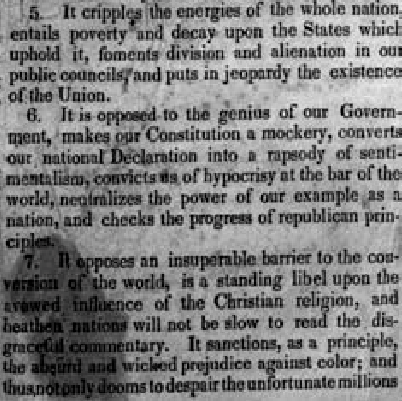
\includegraphics[width=.85\linewidth]{Images/Grayscale.png}
        \caption{Početna crno-bijela slika}
        \label{fig:sub1}
    \end{subfigure}%
    \begin{subfigure}{.5\textwidth}
        \centering
        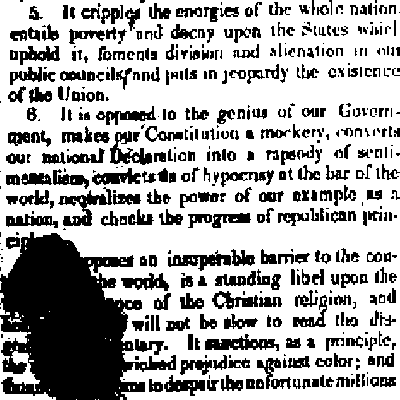
\includegraphics[width=.85\linewidth]{Images/Threshold.png}
        \caption{Slika dobivena binarizacijom fiksnim pragom}
        \label{fig:sub2}
    \end{subfigure}
    \caption{Primjer binarizacije fiksnim pragom}
    \label{fig:threshold}
\end{figure}

\section{Adaptivna binarizacija}
Problemi prikazani u prethodnom postupku rješavaju se primjenom adaptivne binarizacije koja vrijednost sakog pojedinog slikovnog elementa ne određuje samo na osnovu njegove boje, već u obzir uzima i boju okoline.
U nastavku je opisan postupak koji je predložen u \cite{AdaptiveBinarization}.
Prikazani primjeri koriste sliku \ref{fig:sub1} kao početnu.

\subsection{Filtriranje šuma}
Ovisno o stanju dokumenta i načinu digitalizacije istoga moguće je da se na dobivenoj slici pojavljuje šum, kojega je potrebno otkloniti.
Za potrebe opisanoga koristi se niskopropusni Wiener filter \cite{book:Two-Dimensional-Signal-Image-Processing}, koji se temelji na statističkoj procjeni temeljenoj na okruženju svakog pojedinog slikovnog elementa. \cite{AdaptiveBinarization}
Označimo sa $I_s(x, y)$ vrijednost slikovnog elementa početne slike, a sa $I(x, y)$ vrijednost slikovnog elementa filtrirane slike.
Tada se filtrirana slika $I$ može izračunati pomoću formule opisane u knjizi \cite{book:Two-Dimensional-Signal-Image-Processing}:
\[I(x, y) = \mu(x, y) + \frac{\sigma(x, y)^2}{(\sigma(x, y)^2 - v^2)}(I_s(x, y) - \mu(x, y))\]
Sa $\mu(x, y)$ označena je aritmetička sredina vrijednosti slikovnih elemenata u okruženju veličine $NxM$, prema formuli:
\[\mu(x, y) = \frac{1}{NM} 
    \displaystyle \sum_{i = x-\frac{N}{2}}^{x+\frac{N}{2}}
    \displaystyle \sum_{j = y-\frac{M}{2}}^{y+\frac{M}{2}}
I_s(i, j)\]
Sa $\sigma^2$ označena je varijanca vrijednosti slikovnih elemenata u okruženju veličine $NxM$, prema formuli:
\[\sigma(x, y)^2 = \frac{1}{NM} 
    \displaystyle \sum_{i = x-\frac{N}{2}}^{x+\frac{N}{2}}
    \displaystyle \sum_{j = y-\frac{M}{2}}^{y+\frac{M}{2}}
(I_s(i, j)^2 - \mu^2)\]
Sa $v^2$ je označena srednja vrijednost svih lokalnih varijanci.
Konačan rezultat filtriranja, korištenjem okruženja dimenzija $5$x$5$ prikazan je na slici \ref{fig:wiener}.

\begin{figure}[!ht]
\centering
\begin{minipage}{.5\textwidth}
    \centering
    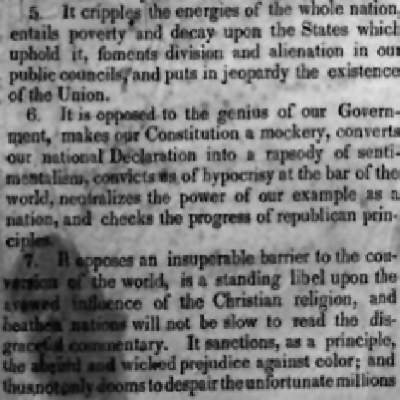
\includegraphics[width=.85\linewidth]{Images/Wiener.png}
    \caption{Slika dobivena filtriranjem šuma}
    \label{fig:wiener}
\end{minipage}%
\begin{minipage}{.5\textwidth}
    \centering
    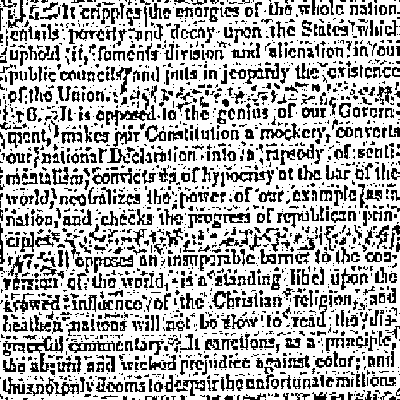
\includegraphics[width=.85\linewidth]{Images/Niblack.png}
    \captionsetup{justification=centering}
    \caption{Slika dobivena korištenjem Niblackovog algoritma adaptivne binarizacije}
    \label{fig:niblack}
\end{minipage}
\end{figure}

\subsection{Procjena sadržaja}
Sljedeći korak binarizacije temelji se na procjenjivanju sadržaja dokumenta. 
Cilj ovog koraka je procijeniti koji elementi slike pripadaju pozadini, a koji pripadaju saržaju dokumenta. 
Pritom je procijenjeni sadržaj zapravo nadskup stvarnog sadržaja, odnosno na dobivenoj slici biti će prisutan šum. 
Za potrebe ovoga koristi se Niblackov algoritam adaptivne binarizacije. \cite{AdaptiveBinarization}\\

Algoritam se temelji na ideji kliznog prozora određenih dimenzija, pomoću kojega se računa lokalni median vrijednosti $m$ te varijanca $s$. 
Kako bi se ubrzao izračun, umjesto mediana se računa aritmetička sredina $\mu$.
Konačan prag binarizacije, $T$, određuje se kao:
\[ T = m + ks \]
gdje je $k$ proizvoljna konstanta koja određuje koliko će okolina trenutnog slikovnog elementa utjecati na prag binarizacije.
Korištena vrijednost je $k = -0.2$.
Konačna slika $N$, dobivena je od početne slike $I$ na sljedeći način:
\[
    N(x, y) =
    \begin{cases}
        1,   & \quad \text{ako je } I(x, y) > T\\
        0,  & \quad \text{inače}\\
    \end{cases}
\]
Rezultati ovog postupka, korištenjem kliznog prozora dimenzija $20$x$20$, uz $k=-0.2$, prikazan je na slici \ref{fig:niblack}.
Na slici se primjećuje kako je sav tekst prepoznat i prikazan crnom bojom, ali je također prisutan i jako izražen šum.

\subsection{Procjena pozadine}
U ovom koraku pokušava se procijeniti izgled pozadine dokumenta, što je označeno sa $B$. 
Za potrebe toga koristi se obrađena početna slika $I$ te prethodno dobivena slika $N$.
Ako je neki slikovni element na slici $N$ označen nulom, taj element predstavlja pozadinu slike i njegova vrijednost na slici $B$ biti će jednaka onoj sa slike $I$.
U protivnome će vrijednost tog slikovnog elementa biti određena interpolacijom vrijednosti susjednih slikovnih elemenata.
Konačna formula za elemente slike $B$ glasi:
\[
    B(x, y) =
    \begin{cases}
        \hfil
        I(x, y),    & \quad \text{ako je } N(x, y) = 0\\[1em]
        \frac{
            \displaystyle \sum_{i = x-dx}^{x+dx}
            \displaystyle \sum_{j = y-dy}^{y+dy}
            (I(i, j)(1 - N(i, j)))
        } {
            \displaystyle \sum_{i = x-dx}^{x+dx}
            \displaystyle \sum_{j = y-dy}^{y+dy}
            (1 - N(i, j))
        }, & \quad \text{ako je} N(x, y) = 1\\

    \end{cases}
\]
Pri čemu $dx$ i $dy$ određuju dimenzije okruženja koje se gleda prilikom interpolacije.
Postupak je u cijelosti objašnjen u radu \cite{AdaptiveBinarization}.\\

\begin{figure}[!ht]
\centering
\begin{minipage}{.5\textwidth}
    \centering
    
\includegraphics[width=.85\linewidth]{Images/Background.png}
    \caption{Slika dobivena procjenom pozadine}
    \label{fig:background}
\end{minipage}%
\begin{minipage}{.5\textwidth}
    \centering
    
\includegraphics[width=.85\linewidth]{Images/FinalThreshold.png}
    \captionsetup{justification=centering}
    \caption{Slika dobivena binarizacijom}
    \label{fig:finalThreshold}
\end{minipage}
\end{figure}

Rezultati ovog postupka, primjenjenog na slici \ref{fig:sub1} prikazani su na slici \ref{fig:background}, uz $dx=3$ i $dy=3$.
Moguće je uočiti kako se na slici i dalje primjećuju obrisi slova, premda sama slova nisu prisutna.

\subsection{Binarizacija}
Kao što je opisano u radu \cite{AdaptiveBinarization}, u ovom koraku se provodi konačna binarizacija, uspoređivanjem izračunate pozadine $B$ i izvorne slike $I$.
Postupak se temelji na tome da je razlika u boji teksta i pozadine veća nego li razlika u boji šuma dobivenog procjenom sadržaja dokumenta i pozadine.
Ovisno o intenzitetu sive boje okruženja, računa se prag binarizacije $d$, kako bi se sačuvao tekst u tamnim područjima.
Kako bi se to postiglo, vrijednost praga $d$ mora biti manja u područjima sa tamnom pozadinom.
Konačna slika $T$ određena je formulom:
\[
    T(x, y) = 
    \begin{cases}
    1,  & \quad \text{ako je } B(x, y) - I(x, y) > d(B(x, y)) \\
    0,  & \quad \text{inače}\\
    \end{cases}
\]
Vrijednost praga, $d(B(x, y))$, moguće je procijeniti kao 
\[d = q * \delta\]
, gdje je $q$ konstanta koja je fiksno postavljena na $0.8$, a $\delta$ se računa kao razlika intenziteta sive boje na početnoj slici za mjesta koja predstavljaju pozadinu i za mjesta koja predstavljaju tekst.
Vrijednost $\delta$ možemo izračunati kao
\[
    \delta = \frac{
        \displaystyle \sum_x
        \displaystyle \sum_y
        (B(x, y) - I(x, y))
    }{
        \displaystyle \sum_x
        \displaystyle \sum_y
        N(x, y)
    }
\]

Konačan rezultat nakon primjene opisanog postupka binarizacije prikazan je na slici \ref{fig:finalThreshold}.
Za razliku od rezultata korištenjem binarizacije sa fiksnim pragom, prikazanim na slici \ref{fig:sub2}, primjećjuje se kako zatamnjeno područje u donjem lijevom kutu slike ne predstavlja problem prilikom raspoznavanja teksta od pozadine.
Također je potrebno primjetiti i šumove koji su ostali prisutni nakon trenutno opisanog postupka, a koji su riješeni u nastavku.

\subsection{Dodatna obrada slike}
Završni korak obrade slike koristi se kako bi se popravila kvaliteta konačne binarizirane slike.
Problemi koji se mogu uočiti na danim primjerima uključuju prisutnost šuma, kao i potencijalne prekide slova, gdje je moguće da neko slovo nije u potpunosti zacrnjeno.\\

\begin{figure}[!ht]
\centering
\begin{minipage}{.5\textwidth}
    \centering
    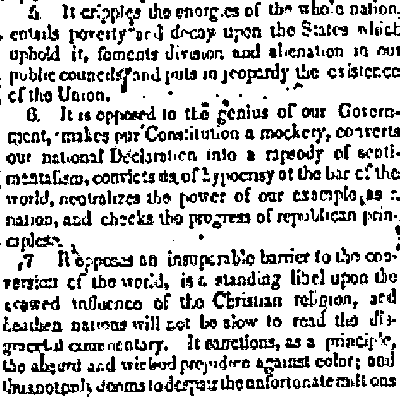
\includegraphics[width=.85\linewidth]{Images/Shrinked.png}
    \captionsetup{justification=centering}
    \caption{Slika dobivena uklanjanjem crnih slikovnih elemenata}
    \label{fig:shrink}
\end{minipage}%
\begin{minipage}{.5\textwidth}
    \centering
    
\includegraphics[width=.85\linewidth]{Images/Swell.png}
    \captionsetup{justification=centering}
    \caption{Slika dobivena uklanjanjem bijelih slikovnih elemenata}
    \label{fig:swell}
\end{minipage}
\end{figure}

Prisutnost šuma se nastoji ukloniti tako što se pregledava cijela slika te se za svaki crni slikovni element provjerava je li on rezultat šuma.
Za potrebe toga koristi se klizni prozor dimenzija $n$x$n$.
U slučaju kada je središnji element kliznog prozora crne boje, prebrojavaju se svi pozadinski (bijeli) slikovni elementi unutar kliznog prozora, što je označeno sa $P_{sh}$.
Ako je $P_{sh} > k_{sh}$, gdje je $k_{sh}$ proizvoljno zadana konstanta, središnji slikovni element se postavlja u bijelu boju.
Na slici \ref{fig:shrink} prikazan je rezultat obrade binarizirane slike navedenim postupkom uz $n = 5$ i $k_{sh} = 0.8$.
Primjećuje se kako i dalje postoje smetnje na slici, no problem nastaje kod toga što bi niža vrijednost parametra $k_{sh}$ osigurala bolje uklanjanje šumova, ali bi istovremeno povećala vjerojatnost da se uklone elementi teksta, što nije poželjno.\\

Drugi korak spomenut u ovom postupku provodi se slično kao i prethodni.
Potrebno je prebrojati broj crnih slikovnih elemenata, $P_{sw}$, koji se nalaze unutar kliznog prozora dimenzija $n$x$n$.
Ako je srednji element bijel i vrijedi $P_{sw} > k_{sw}$, središnji se element pretvara u crni.
Postupak je demonstriran na slici \ref{fig:swell}, uz $n = 5$ i $k_{sw} = 0.6$.


\chapter{Prepoznavanje zakrivljenosti slike}
Jedan od problema koji nastaje prilikom digitalizacije dokumenata je mogućnost da dokument bude nakošen. 
Do toga može doći ili prilikom nepažnje tokom ubacivanja papira u optički čitač, ili zbog nesvjesnog zakrivljenja prilikom korištenja kamere mobilnog uređaja.
Nakošenost digitalizirane slike može uzrokovati teže ili lošije prepoznavanje elemenata na slici, zbog čega je korisno i poželjno otkriti stupanj rotacije dokumenta i ispraviti ga.

\section{Računanje kuta rotacije}
Počevši od dokumenta kakav je prikazan na slici \ref{fig:skew_original}, može se uočiti kako se na njemu jasno prepoznaju vodoravne linije dokumenta.
Unatoč činjenici da to nije opći slučaj koji uvijek vrijedi, u ovom radu nije razrađeno kako općeniti dokument svesti na ovakav oblik, već se kreće od pretpostavke da će dokument uvijek imati jasno izražene linije, bilo vodoravne, bilo okomite.
Ova pretpostavka vrijedi isključivo iz razloga da se rad fokusira na prepoznavanje tablica na skeniranim dokumentima.\\

\begin{figure}[ht!] 
    \centering
    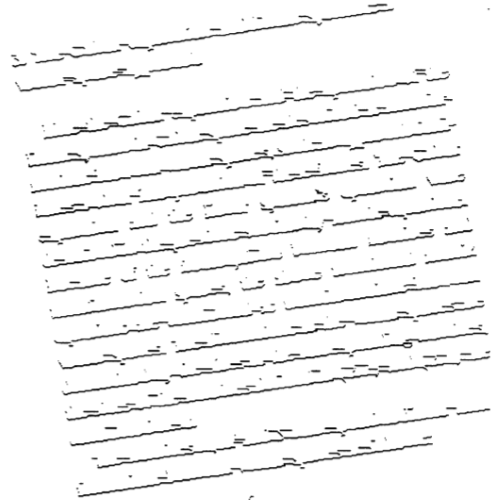
\includegraphics[width=.4\textwidth]{Images/Skew_original.png}
    \captionsetup{justification=centering}
    \caption{Početni nakošeni dokument\cite{article:Skew-detection}}
    \label{fig:skew_original}
\end{figure}

Temeljna ideja koja se koristi prilikom izračuna kuta rotacije je ta da se dokument presječe okomitim linijama, što je predloženo u radu \cite{article:Skew-detection}.
Za svaku okomitu liniju se računaju točke u kojima ona sječe linije osnovnog dokumenta.
Jednom kada su određene točke sjecišta, moguće je odabrati jednu takvu točku najljevije okomite linije ($T_1$) te usporediti tu točku sa svim točkama koje se nalaze desno od nje ($T_2$).
Dvije tako odabrane točke analiziraju se na način da se kroz njih povuče pravac, čija jednadžba glasi: 
\[
    y - y_1 = k(x - x_1),
\]
gdje je $k$ koeficjent smjera:
\[
    k = \frac{y_2 - y_1}{x_2 - x_1}.
\]
Pomoću koeficjenta smjera $k$ moguće je izračunati kut pod kojim je nagnut dobiveni pravac, kao $\alpha = tan^{-1}(k)$.
Uz pretpostavku da dokument nije rotiran te da se točke $T_1$ i $T_2$ nalaze na istim vodoravnim linijama dokumenta, kut $\alpha$ trebao bi iznositi $0\degree$.
U slučaju da je dokument rotiran, ovako određen kut $\alpha$ biti će jednak stupnju rotacije dokumenta.\\

\begin{figure}[th!]
    \centering
    \begin{subfigure}{.5\textwidth}
        \centering
        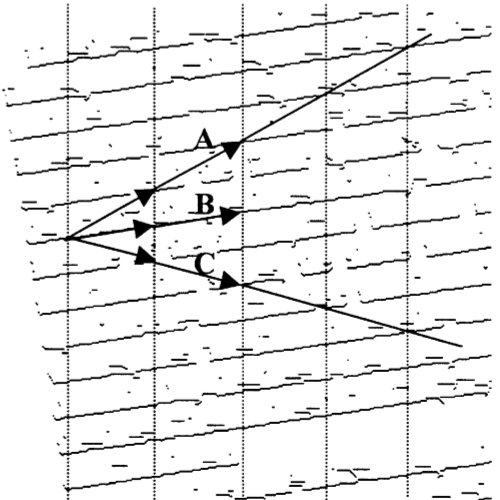
\includegraphics[width=.85\linewidth]{Images/Skew_equidistant.png}
        \captionsetup{justification=centering}
        \caption{Dokument podijeljen ekvidistantnim linijama\cite{article:Skew-detection}}
        \label{fig:skew_equidistant}
    \end{subfigure}%
    \begin{subfigure}{.5\textwidth}
        \centering
        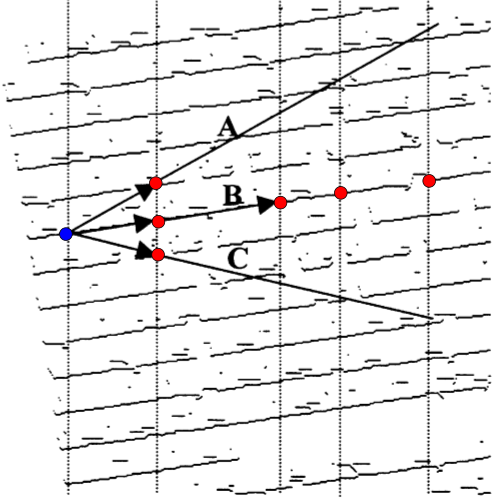
\includegraphics[width=.85\linewidth]{Images/Skew_random.png}
        \captionsetup{justification=centering}
        \caption{Dokument podijeljen linijama sa nasumičnim udaljenostima\cite{article:Skew-detection}}
        \label{fig:skwe_random}
    \end{subfigure}
    \caption{Primjer podjele dokumenta okomitim linijama}
    \label{fig:skew_verticalLines}
\end{figure}

Jedan od problema koji preostaje je početna pretpostavka da se točke $T_1$ i $T_2$ nalaze na istoj vodoravnoj liniji dokumenta, što neće biti istinito u većini slučajeva.
To se rješava na način da se izračunaju kutevi koje zatvaraju svi pravci koji počinju u točki $T_1$, a pritom se bilježi koliko puta se pojavio koji kut.
Uz ovaj pristup rotaciju dokumenta više ne određuje kut $\alpha$ koji je dobiven za jedan pravac, već onaj kut koji je najviše puta zabilježen.
Ovaj pristup prikazan je na slici \ref{fig:skew_verticalLines}, gdje je za određenu podjelu okomitim linijama i odabranu početnu točku prikazan izračun triju kuteva: \textbf{A}, \textbf{B}, \textbf{C}.
Slika \ref{fig:skew_equidistant} također prikazuje i važnost načina odabira okomitih linija.
Na navedenoj slici odabrane su ekvidistantne linije, zbog čega dolazi do toga da se sva tri kuta javljaju jednak broj puta, što ometa rad algoritma.
Za razliku od toga, na slici \ref{fig:skwe_random} koriste se linije sa nasumičnim međusobnim udaljenostima te se primjećuje kako se na njoj kut \textbf{B} javlja prilikom svakog presjeka okomite linije sa vodoravnom linijom na kojoj se nalazi početna točka $T_1$, dok se ostali kutevi javljaju samo jednom, čime se prepoznaje da oni dolaze radi krivo odaranih točaka.


\section{Rezultati}
Kako bi se uštedjelo na vremenu izvođenja, navedeni algoritam je implementiran na način da nakon što odredi nasumične okomite linije odabire samo $4$ početne točke, prethodno označene sa $T_1$.
Za te točke se računaju kutevi sa svim ostalim točkama, a na kraju se provjerava postoji li kut koji prevladava.
Primjer jednog takvog izvođenja prikazan je na slici \ref{fig:skew1}.\\

\begin{figure}[ht!]
    \centering
    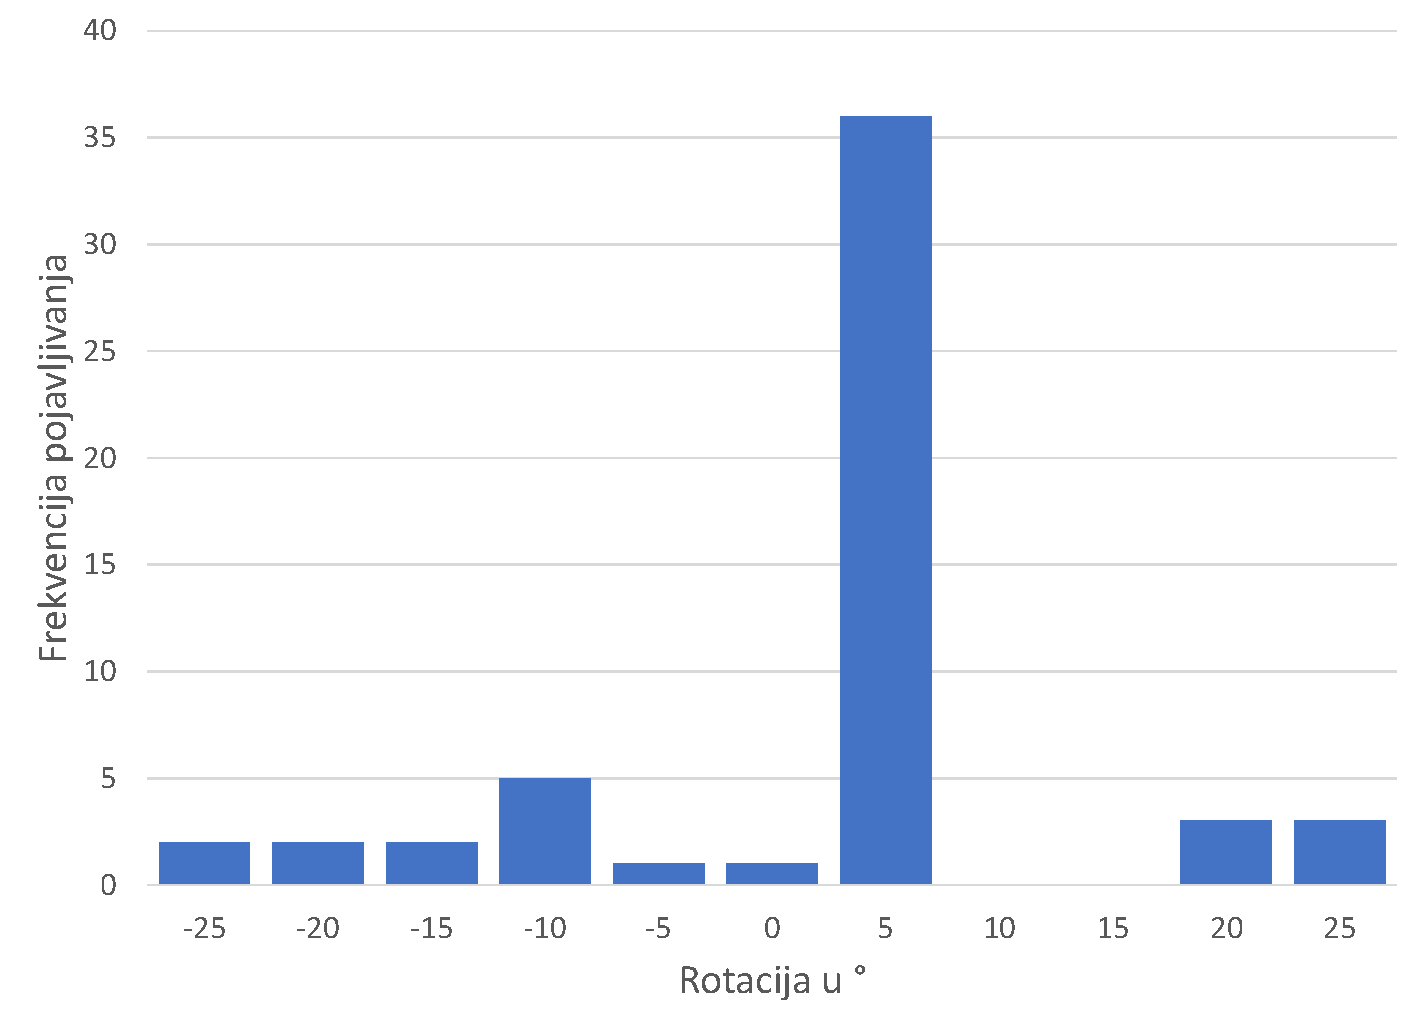
\includegraphics[width=.8\textwidth]{Images/Skew1.pdf}
    \captionsetup{justification=centering}
    \caption{Histogram s prikazom frekvencija pojavljivanja kuteva}
    \label{fig:skew1}
\end{figure}

Iz slike se može lako primjetiti kako je najčešće izmjeren kut od $5\degree$ stupnjeva, iz čega se zaključuje da je slika rotirana za točno taj iznos.
Isti postupak ponovljen je za sliku koja je bila rotirana za kut od $10\degree$ stupnjeva, a rezultati toga prikazani su histogramom na slici \ref{fig:skew2}.
Na ovoj slici se primjećuje kako se za veće iznose kuteva javlja veći šum u izračunatim kutevima, no i dalje je moguće razaznati dominantnu vrijednost kuta rotacije.\\

\begin{figure}[ht!]
    \centering
    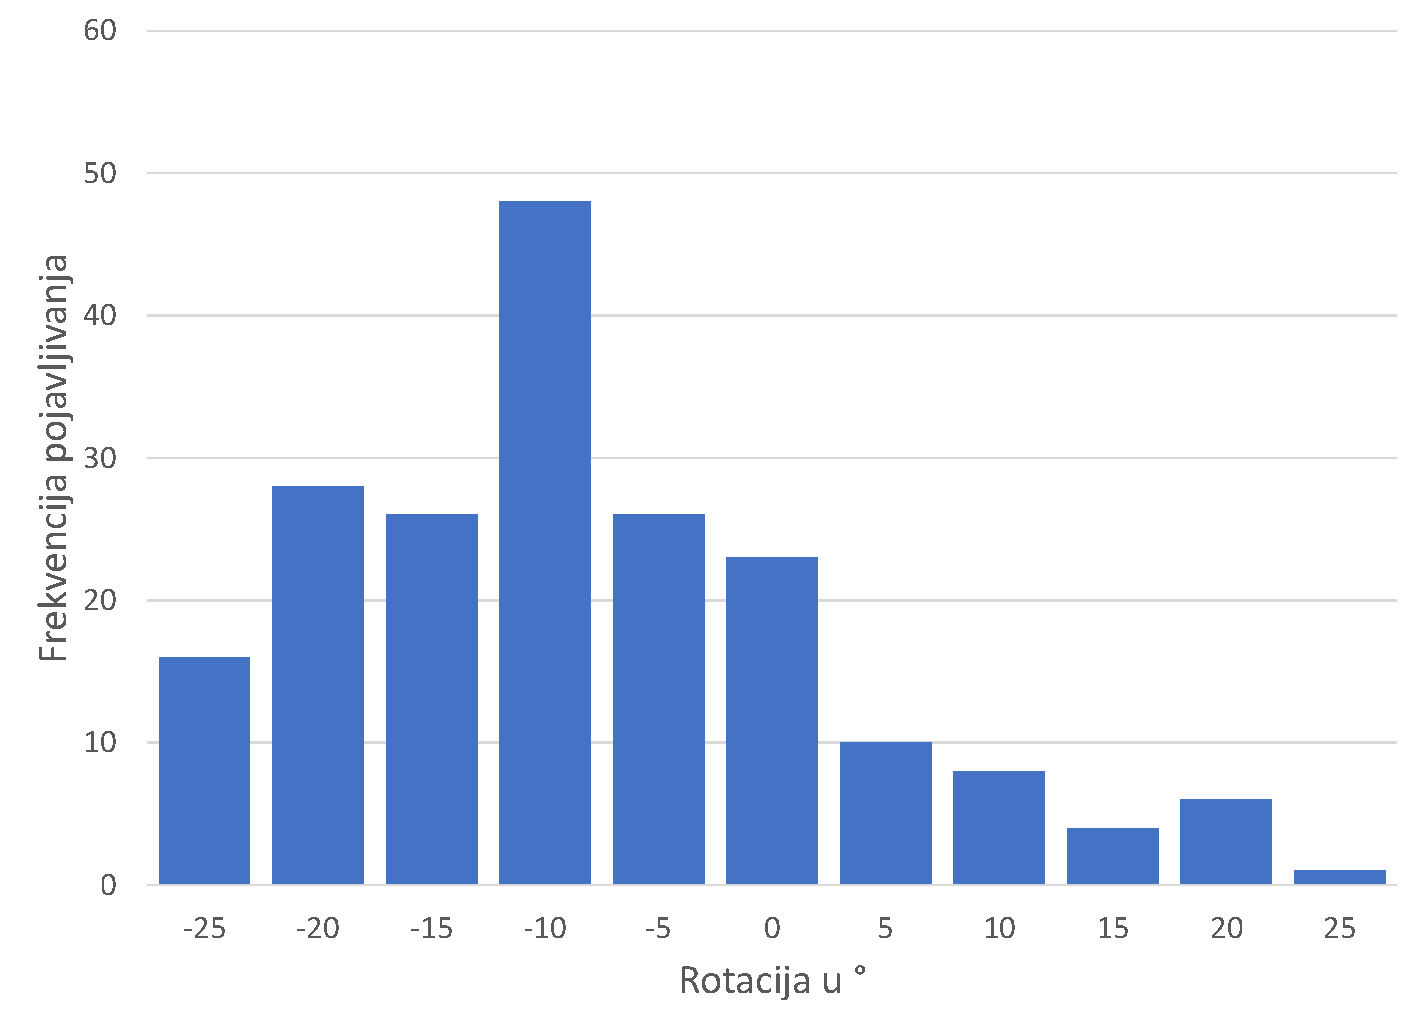
\includegraphics[width=.8\textwidth]{Images/Skew2.pdf}
    \captionsetup{justification=centering}
    \caption{Histogram s prikazom frekvencija pojavljivanja kuteva}
    \label{fig:skew2}
\end{figure}

Problem se javlja kod izračuna koji je prikazan histogramom na slici \ref{fig:skew3}, gdje nije moguće sa sigurnošću odrediti kako je slika rotirana.
Do ovog problema je moglo doći iz više razloga, poput loše odabranih okomitih linija, ili problema zbog točaka dobivenih kao sjecišta okomitih linija i teksta koji se nalazi u tablicama.
Jednostavno i efikasno rješenje navedenog problema je ponovno određivanje okomitih linija te ponovan izračun kuteva sa nove proizvoljne $4$ točke.

\begin{figure}[ht!]
    \centering
    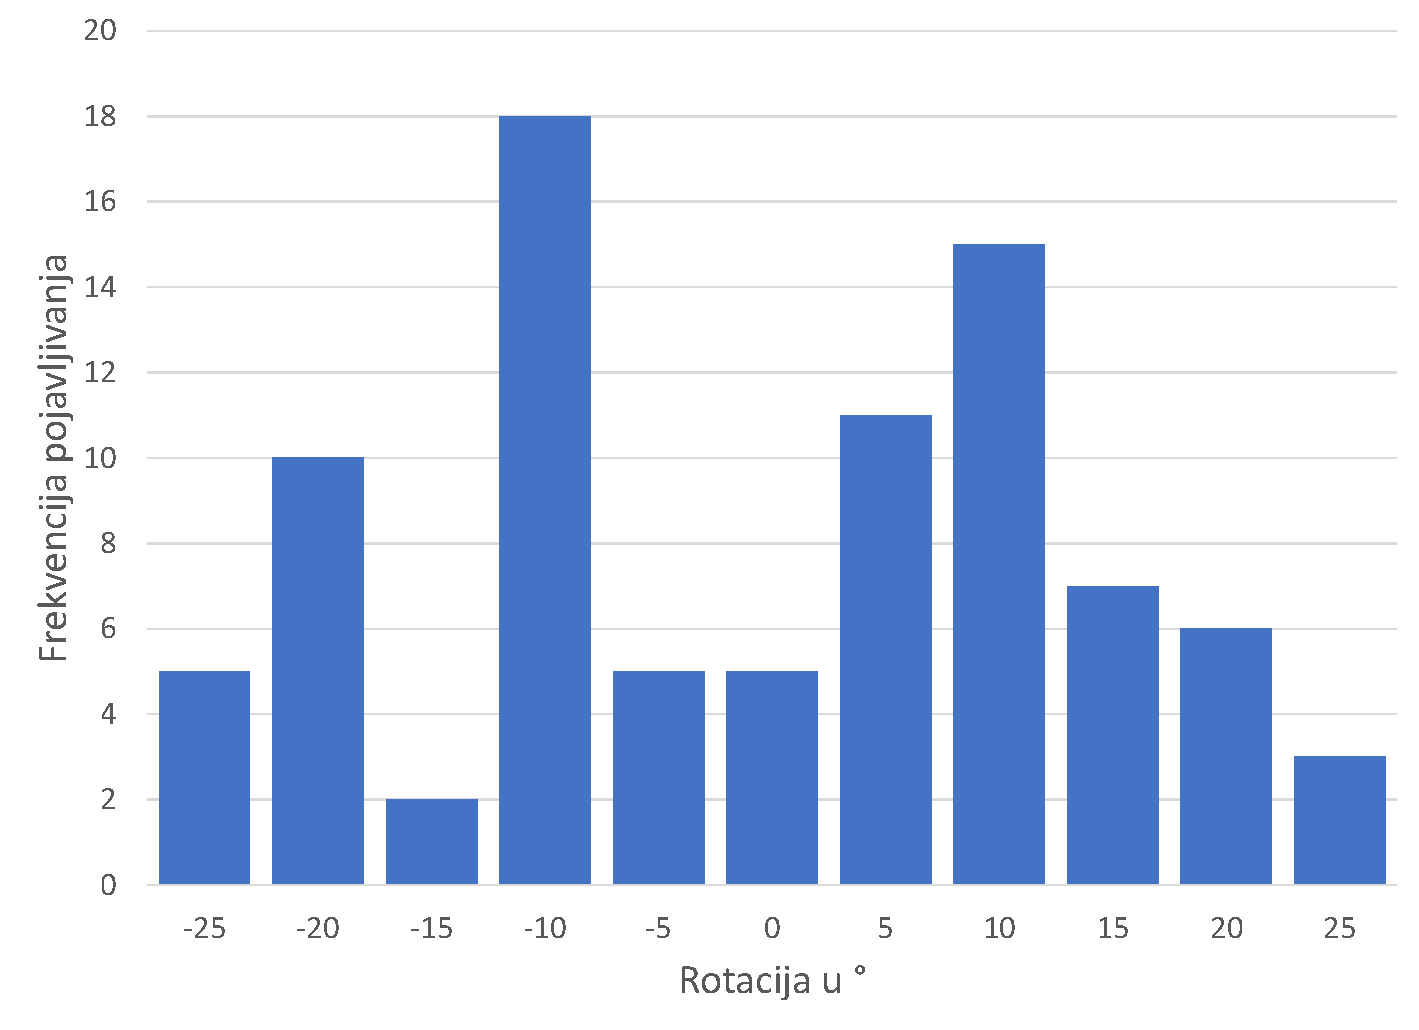
\includegraphics[width=.8\textwidth]{Images/Skew3.pdf}
    \captionsetup{justification=centering}
    \caption{Histogram s prikazom frekvencija pojavljivanja kuteva}
    \label{fig:skew3}
\end{figure}

\chapter{Detekcija tablice}
Kao što je predloženo u radu \cite{conference:AutomaticTableDetectionInDocumentImages}, detekcija tablice temelji se na detekciji vrhova ćelija. 
Analiziranjem općenitih tablica, moguće je uočiti kako postoji $9$ različitih mogućnosti koje se mogu pojaviti kao vrh ćelije, što je prikazano na slici \ref{fig:corners}.

\begin{figure}[ht!]
    \centering
    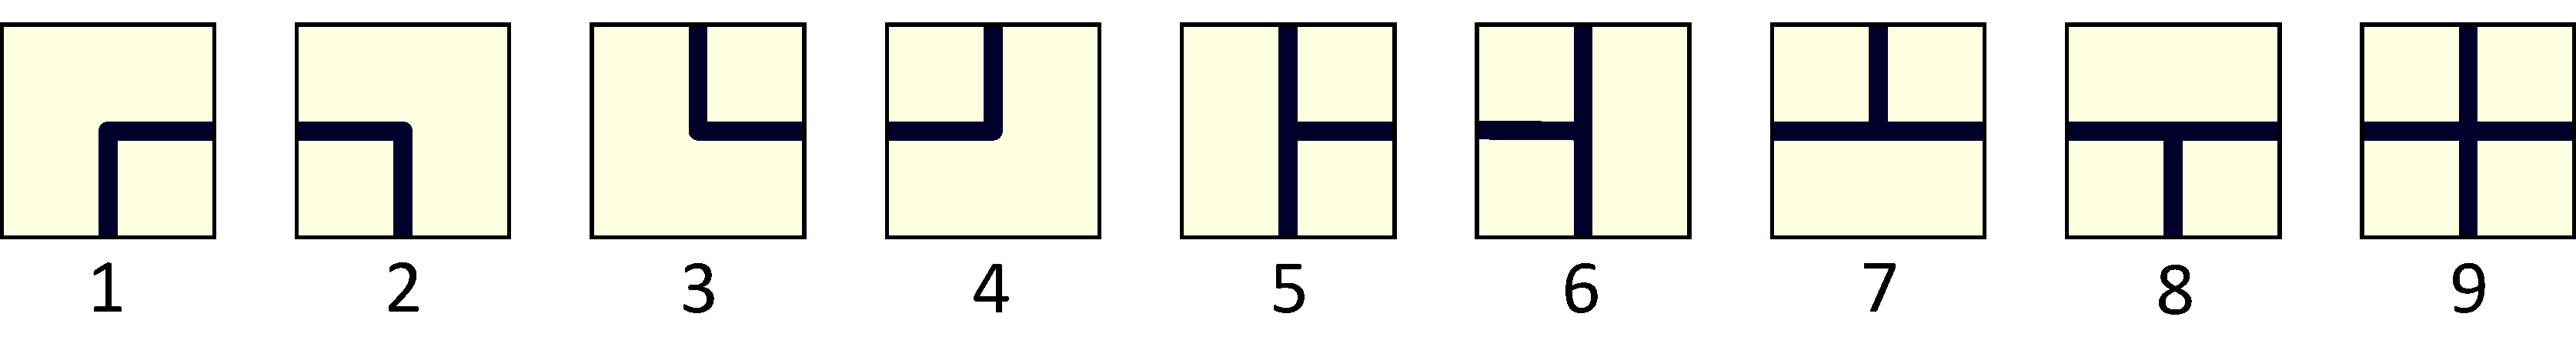
\includegraphics[width=1.0\textwidth]{Images/Corners.pdf}
    \captionsetup{justification=centering}
    \caption{Prikaz mogućih vrsta vrhova ćelija}
    \label{fig:corners}
\end{figure}

Prve $4$ mogućnosti sa slike predstavljaju vrhove ćelija koje su ujedno i vrhovi cijele tablice. 
Sljedeće $4$ mogućnosti izgleda vrha ćelija predstavljaju rubove tablice, odnosno početak ili kraj linija tablice.
Zadnja prikazana mogućnost predstavlja sjecišta linija koja se nalaze unutar tablice.
Detektiranjem točnih pozicija ovih $9$ elemenata te točnom klasifikacijom istih, moguće je jednoznačno rekonstruirati tablicu.\\

Pretragu je moguće ubrzati korištenjem znanja o općem izgledu tablice.
U skladu s time je moguće pronaći isključivo pozicije prve $4$ vrste vrhova, na temelju čega se određuju rubovi tablice.
Koristeći te informacije moguće je odrediti vanjski obrub tablice, na kojemu se moraju nalaziti svi oblici označeni sa $5-8$ na slici \ref{fig:corners}, te nije potrebno pretraživati ostatak slike i vršiti klasifikaciju pronađenih kandidata.
Nakon što se pronađu tako opisani rubovi, vrh označen brojem $9$ na slici može se locirati kao sjecište linija između prethodno definiranih rubova tablice.
Ovaj pristup nije detaljnije razrađen u ovom radu te nije korišten u implementaciji, a navodi se isključivo kao prijedlog potencijalne optimizacije korištenog algoritma.

\section{Detekcija vrhova ćelija}
Detekcija vrhova ćelija obavlja se na način da se svaki dio slike provjerava te se za njega utvrđuje prikazuje li on vrh ćelije ili ne. 
Kako bi se to izvelo, potrebno je odrediti točno koji dio slike se provjerava u nekom određenom trenutku, a što se čini korištenjem pomičnog prozora. 
Definiran je prozor određenih dimenzija $X$x$Y$, te se promatra samo dio slike unutar njega. 
Tako dobiven isječak slike potom se analizira i ispituje sadrči li on vrh ćelije ili ne.
Jednom kad je detekcija završena za trenutni prozor, prozor se pomiče po $x$ osi za udaljenost $dx$, te se detekcija vrši na tako dobivenom novom isječku slike.
Jedno od mogućih poboljšanja ove metode predloženo je u radu \cite{ViolaJones}, gdje se ne koristi fiksna veličina pomičnog prozora, već se pretraga započinje s jednom veličinom prozora te se ona iterativno smanjuje tokom pretrage.


\subsection{Određivanje značajki}
Prije nego li se može napraviti detekcija vrhova, potrebno je definirati značajke prema kojima se isti pretražuju.
Osnovna funkcija značajki je pojednostavljenje slike koja se pokušava prepoznati kako bi se smanjio ukupan prostor stanja pretrage.
Potrebno je odrediti značajke koje vrijede neovisno o manjim pomacima slike, ili manjim šumovima koji mogu biti prisutni iz različitih razloga.
Za potrebe toga odabrana su dva različita pristupa odabira značajki.\\

Prvi korišteni način zasniva se na činjenici da se detektiraju djelovi tablica, koje se sastoje isključivo od vodoravnih i okomitih linija.
Imajući to na umu moguće je uočiti da će u idealnom slučaju okomite i vodoravne zrake (prikazano crvenom bojom) sjeći vrh ćelije uvijek u samo jednoj točki, kao što je prikazano u primjeru na slici \ref{fig:lineFeatures}.

\begin{figure}[th!]
    \centering
    \begin{subfigure}{.5\textwidth}
        \centering
        
\includegraphics[width=.3\linewidth]{Images/LineFeature.pdf}
        \captionsetup{justification=centering}
        \caption{Primjer zrake bez sjecišta}
        \label{fig:feature1}
    \end{subfigure}%
    \begin{subfigure}{.5\textwidth}
        \centering
        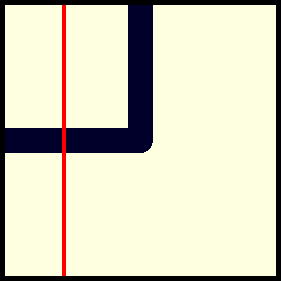
\includegraphics[width=.3\linewidth]{Images/LineFeature1.pdf}
        \captionsetup{justification=centering}
        \caption{Primjer zrake sa sjecištem}
        \label{fig:feature2}
    \end{subfigure}
    \caption{Primjer ekstrakcije značajki korištenjem okomite zrake}
    \label{fig:lineFeatures}
\end{figure}

Ovisno o koordinati zrake moguće je odrediti koja je to vrsta vrha, točnije na danom primjeru na slici \ref{fig:feature1} nema sjecišta zrake i linije, iz čega se zaključuje kako se na slici ne nalaze određeni vrhovi ćelija, poput na primjer vrha označenog brojem $2$ na slici \ref{fig:corners}, koji ima vodoravnu liniju na lijevoj strani.
Ista ta zraka na primjeru na slici \ref{fig:feature2} presjeca sliku na jednom mjestu, iz čega se zaključuje da je na slici potencijalno vrh koji na tom mjestu ima liniju.\\

Ovaj pristup se nadopunjuje na način da se umjesto broja presjecišta određuje udaljenost od prvog presjecišta.
Na taj se način razlikuje linija koja se očekivano pojavljuje na sredini slike od šuma koji se može pojaviti na svim mjestima slike.
Prilikom ovog pristupa koji uključuje izračun udaljenosti do presjecišta potrebno je relativizirati dobivenu udaljenost u odnosu na veličinu slike na kojoj se radi analiza kako bi se osiguralo da značajke ne ovise o veličini slike.
Osim navedenoga, koriste se i dijagonalne zrake s kojima se određuje broj presjecišta kako bi se dodatno povećala raznolikost značajki, a samim time i robusnost algoritma.\\

Drugi pristup određivanja značajki slike temelji se na pristupu koji je korišten u radu \cite{ViolaJones}.
Ove značajke temelje se na činjenici da različiti dijelovi slike sadrže različitu količinu crnih slikovnih elemenata.
Kao što je prikazano na slici \ref{fig:haarFeatures}, gdje su prikazana $4$ različita oblika značajki ovog tipa koje se koriste u ovome radu, značajke se gledaju za određeni dio slike, što je prikazano pravokutnikom.
Vrijednost značajke se računa kao razlika broja crnih slikovnih elemenata u crnom i bijelom djelu pravokutnika.
Kako bi se postigla neovisnost o veličini slike nad kojom se vade značajke, izračunata razlika broja slikovnih elemenata dijeli se ukupnim brojem slikovnih elemenata u kvadratu značajke.
Na ovaj način se ispituje je li neko područje tamnije od njemu susjednog područja, što je primjer kod linija tablice, gdje se linija prolazi sredinom promatranog područja koje je zbog toga tamno, a neposredno pored nje se nalazi bijelo područje. 
Potencijalne smetnje koje mogu nastati na slici kao posljedica sadržaja tablice ne utječu značajno na vrijednost značajke, budući da značajka obuhvaća veću površinu, a potencijalne smetnje se u većini slučajeva nalaze na manjem lokalnom području.

\begin{figure}[th!]
    \centering
    \begin{subfigure}{.25\textwidth}
        \centering
        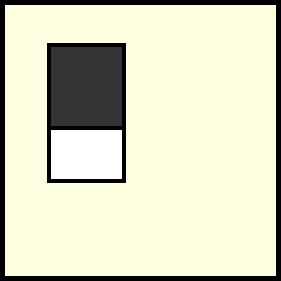
\includegraphics[width=.5\linewidth]{Images/Haar_VD.pdf}
        \captionsetup{justification=centering}
        \caption{}
        \label{fig:haar1}
    \end{subfigure}%
    \begin{subfigure}{.25\textwidth}
        \centering
        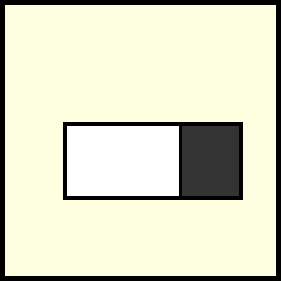
\includegraphics[width=.5\linewidth]{Images/Haar_HD.pdf}
        \captionsetup{justification=centering}
        \caption{}
        \label{fig:haar2}
    \end{subfigure}%
    \begin{subfigure}{.25\textwidth}
        \centering
        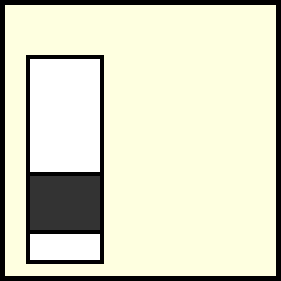
\includegraphics[width=.5\linewidth]{Images/Haar_VT.pdf}
        \captionsetup{justification=centering}
        \caption{}
        \label{fig:haar3}
    \end{subfigure}%
    \begin{subfigure}{.25\textwidth}
        \centering
        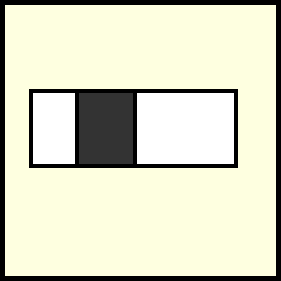
\includegraphics[width=.5\linewidth]{Images/Haar_HT.pdf}
        \captionsetup{justification=centering}
        \caption{}
        \label{fig:haar4}
    \end{subfigure}
    \caption{Primjeri značajki temeljenih na razlici količine boje}
    \label{fig:haarFeatures}
\end{figure}

Prednost ovog skupa značajki je u mogućnosti izračuna istih u konstantnoj složenosti, uz prethodno predprocesiranje podataka.
Računa se novi oblik reprezentacije slike ($ii$) u kojemu je vrijednost na poziciji $x, y$ jednaka ukupnom broju crnih slikovnih elemenata na početnoj slici za sve elemente koji se nalaze gore lijevo od trenutnog, odnosno:
\[
    ii(x, y) = 
        \displaystyle \sum_{x' < x} 
        \displaystyle \sum_{y' < y}
        i(x', y')
\]

\begin{figure}[ht!]
    \centering
    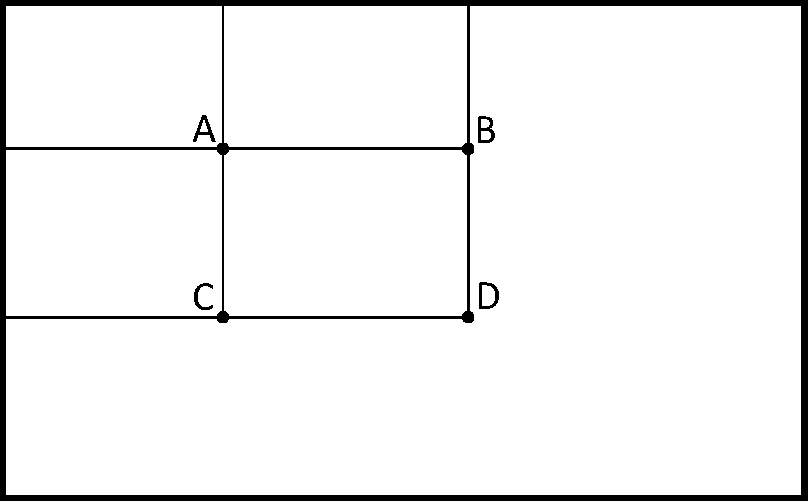
\includegraphics[width=0.5\textwidth]{Images/Integral.pdf}
    \captionsetup{justification=centering}
    \caption{Primjer izračuna broja crnih elemenata unutar kvadrata}
    \label{fig:integral}
\end{figure}

Ove vrijednosti je moguće izračunati jednim prolazom kroz početnu sliku. 
Korištenjem ovih suma moguće je izračunati broj crnih elemenata za bilo koji kvadrat na početnoj slici.
Primjer izračuna prikazan je slikom \ref{fig:integral}, na kojoj je prikazan kvadrat $ABCD$ za kojega želimo izračunati opisanu vrijednost. 
Važno je uočiti da su prethodno već izračunate sume od gornjeg lijevog kuta do svake pojedine točke.
Traženu vrijednost je moguće prikazati kao kumulativnu sumu u točki $D$, što uključuje cijeli kvadrat, kao i područja lijevo i iznad njega.
Vrijednost područja koje se nalazi lijevo od kvadrata jednaka je sumi u točki $C$ te se ta vrijednost oduzima od prethodne vrijednosti.
Analogno tome, od trenutne vrijednosti oduzima se suma u točki $B$.
Trenutni postupak je u dva navrata oduzeo vrijednost područja koje se nalazi gore lijevo od točke $A$ pravokutnika, zbog čega je potrebno trenutnoj vrijednosti jednom pridodati sumu u točki $A$.
Konačna vrijednost za dani kvadrat glasi:
\[
    f = ii(D_x, D_y) - ii(C_x, C_y) - ii(B_x, B_y) + ii(A_x, A_y)
\]

\subsection{Detekcija korištenjem umjetne neuronske mreže}
Umjetne neuronske mreže nastale su kao model kojim se nastoji simulirati način rada ljudskog mozga.
U nastavku je ukratko opisan način rada istih, dok se detaljnije objašnjenje može pronaći u knjizi \cite{umjetnaInteligencija}.
Poznato je da se mozak sastoji od velikog broja međusobno povezanih neurona.
Svaki se neuron sastoji od $3$ djela: dendrita koji primaju električne podražaje, tijela koje reagira na podražaj i aksona koji prosljeđuje podražaj sljedećim povezanim neuronima.
Osnovni princip rada neurona temelji se upravo na spomenutoj propagaciji električnih impulsa. 
Umjetni neuroni simuliraju pojednostavljeni model bioloških neurona na način da oponašaju prethodno navedene funkcionalnsti.

\begin{figure}[ht!]
    \centering
    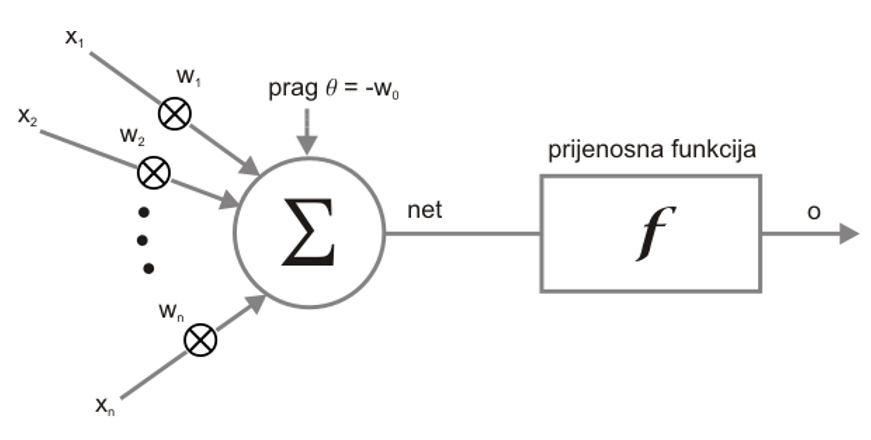
\includegraphics[width=0.5\textwidth]{Images/Neuron.png}
    \captionsetup{justification=centering}
    \caption{Prikaz modela umjetnog neurona}
    \label{fig:neuron}
\end{figure}

Slika \ref{fig:neuron} prikazuje opći model takvog neurona. 
Ulazne vrijednosti neuronu čine vrijednosti od $x_1$ do $x_n$, te se svakoj od njih dodijeljuje određena težina $w_1$ do $w_n$ sa kojom se ulazna vrijednost množi.
Na taj se način ostvaruje mogućnost postavljanja različitih prioriteta različitim ulazima.
Tijelo neurona ostvareno je funkcijom sumacije koja zbraja težinske vrijednosti ulaza te tako dobiveni broj predaje prijenosnoj funkciji, koja se ponaša kao model aksona.
Prijenosna funkcija za dani argument vraća rezultat iz određenog raspona, što se propagira kao ulaz sljedećim neuronima.\\

Korištenjem samo jednog neurona moguće je ostvariti jednostavnije linearne klasifikacijske algoritme, na način da se kao ulazi neurona koriste značajke prema kojima se klasificira, a za prijenosnu funkciju odabere funkcija skoka.
Ovisno o izlazu iz neurona uzorak se klasificira u jedan od dva rezreda.
Prvi nedostatak ovog modela koji se uočava je nemogućnost istoga da uzorak klasificira ako postoji više različitih razreda.
Taj se problem može riješiti dodavanjem novih neurona koji primaju jednake ulaze kao i prvi neuron, te izlaz svakog od njih odgovara pojedinom razredu u koji ulazni uzorak može biti klasificiran.
Takva grupacija neurona zove se sloj neuronske mreže.\\

Sljedeći problem dobivenog modela je mogućnost rada isključivo sa linearno odvojivim podatcima. Taj se problem rješava dodavanjem novih slojeva neurona u neuronsku mrežu, na način da se izlazi neurona jednog sloja proslijede kao ulazi neuronima drugog sloja.
Pri tome se razlikuju $3$ općenite vrste slojeva: ulazni sloj neurona koji služi kako bi se ulazne vrijednosti značajki prosliejdile ostatku neuronske mreže, skriveni sloj neurona koji se koristi prilikom računanja, ali nije vidljiv vanjskom korisniku te izlazni sloj, čiji se rezultat predaje krajnjem korisniku.

\begin{figure}[ht!]
    \centering
    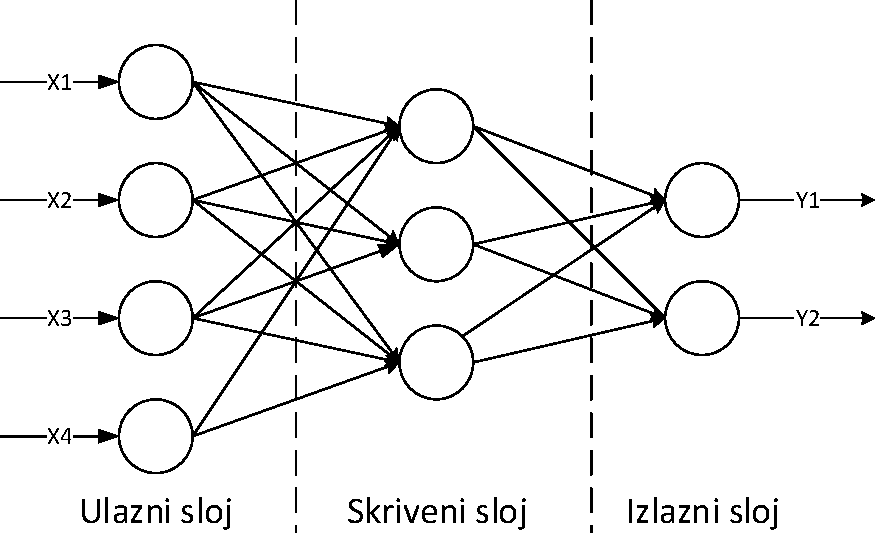
\includegraphics[width=0.7\textwidth]{Images/FFANN.pdf}
    \captionsetup{justification=centering}
    \caption{Model unaprijedne neuronske mreže}
    \label{fig:ffann}
\end{figure}

Ovisno o načinu povezivanja neurona moguće je ostvariti različite arhitekture umjenih neuronskih mreža. 
U radu je korištena unaprijedna neuronska mreža, kakva je prikazana na slici \ref{fig:ffann}.
Jedna od prednosti umjetnih neuronskih mreža leži u mogućnosti učenja istih, a što je moguće učiniti promjenom težina ulaza za pojedini neuron.
Jednom kad je mreža naučena, odnosno kada su određene težine uz koje mreža zadovoljavajuće izvršava zadatak za koji je predviđena, dobiene težine pohranjuju se u datoteku na računalu kako se a daljnja pokretanja mreža ne bi morala ponovno učiti.
Ovo svojstvo omogućava veliku brzinu klasifikacije jednom kada je mreža naučena.

\subsection{Detekcija AdaBoost algoritmom}
Umjetne neuronske mreže izvode velik broj računskih operacija kako bi klasificirale neki ulazni primjer.
To predstavlja problem kada je potrebno klasificirati velik broj uzoraka, kao što je to slučaj kod detekcije vrhova ćelija, gdje je potrebno za svaki mogući element slike odrediti je li on vrh ćelije ili ne.
Kako bi se taj postupak ubrzao koristi se drugačiji pristup klasificiranju primjenom bržih algoritama. \\

Osnovna ideja AdaBoost algoritma je izgraditi jedan jaki klasifikator primjenom više slabih klasifikatora.
U okviru ovog algoritma, jaki klasifikator je finalni klasifikator koji uz veliku točnost podatke raspoređuje u jednu od grupa, dok su slabi klasifikatori u stanju točno klasificirati samo manji podskup podataka, dok ostale svrstavaju u krive grupe.\\

Slabi klasifikatori određuju fiksni prag za kojega će nešto klasificirti u jednu ili drugu kategoriju, ovisno o vrijednosti korištene značajke za sliku. Takav klasifikator prikazan je sljedećom funkcijom:
\[
    h(x, f, p, \theta) = 
    \begin{cases}
    1,  & \quad \text{ako je } pf(x) < p\theta \\
    0,  & \quad \text{inače}\\
    \end{cases}
\]
gdje je sa $h(x, f, p, \theta)$ označen klasifikator, sa $x$ uzorak, sa $f$ funkcija koja na temelju uzorka određuje značajku, a $p$ predstavlja faktor koji određuje smjer nejednakosti, ovisno o predznaku.
Ukupna greška ovakvog klasifikatora definirana je kao težinska suma svih odstupanja, gdje se svakom uzorku pridjeluje određena težina kojom on doprinosi ukupnoj grešci.
Izračun ukupne greške $\epsilon$ prikazan je formulom:
\[
    \epsilon = \displaystyle \sum_{i}w_i \abs{h(x, f, p, \theta) - y_i} 
\]
gdje je sa $w_i$ predstavljena težina $i$-tog po redu uzorka, a sa $y_i$ očekivana vrijednost izlaza klasifikatora.\\

Jaki klasifikatori grade se kao spoj više slabih klasifikatora na način da se računa izlaz svakog od njih te se na temelju toga donosi konačna odluka o kategoriji u koju treba svrstati ulazni uzorak.
Kako bi se stvorio jaki klasifikator potrebno je odrediti skup labeliranih ulaznih primjera koji se koriste tokom učenja.
Budući da algoritam može klasificirati samo $2$ kategorije podataka, potrebno mu je predati uzorke koje smije i koje ne smije prepoznati, gdje je sa $1$ označen uzorak koji se prepoznaje, a sa $0$ uzorak koji se ne prepoznaje.
Na slučaju tablica, algoritam prepoznaje sve obliek vrhova ćelija, a pritom ne prepoznaje sadržaj unutar tablice, linije tablice i ostale smetnje koje se pojavljuju na slici.
Početne težine za svaki od uzoraka postavljene su na: 
\[
    w_i = 
    \begin{cases}
    \frac{1}{m}, & \quad y_i = 0\\
    \frac{1}{l}, & \quad y_i = 1\\
    \end{cases}
\]
Pritom je sa $m$ označen broj negativnih uzoraka, a sa $l$ broj pozitivnih uzoraka.
Potom se ovisno o željenom broju slabih klasifikatora ponavlja sljedeći postupak.
Prvo je potrebno normalizirati sve težine:
\[
    w_i \leftarrow \frac{w_i}{
        \displaystyle \sum_{j = 1}^{n}w_j
    }
\]
Potom se određuje slabi klasifikator $h$ koji za trenutne težine daje najmanju pogrešku $\epsilon$, izračunatu na prethodno opisani način.
Dobiveni slabi klasifikator nije u mogućnosti točno klasificirati određeni dio podataka, zbog čega je potrebno postići da sljedeći slabi klasifikator uspješno prepozna te podatke.
To se postiže mijenanjem trenutnih težina korištenih u izračunu greške na način da se povećavaju težine onih ulaza čija je vrijednost pogrešno klasificirana, a smanjuju težine ulaza čija je vrijednost ispravno klasificirana, prema formuli:
\[
    w_i \leftarrow 
    \begin{cases}
        w_i\beta, & \quad \text{ako je uzorak $i$ točno klasificiran}\\
        w_i, & \quad \text{inače}\\
    \end{cases}
\]
Pritom je koeficjent $\beta$ definiran kao: 
\[
    \beta = \frac{\epsilon}{1 - \epsilon}
\]
Za ovako određen slabi klasifikator računa se još i vrijednost $\alpha$ kao: 
\[
    \alpha = log(\frac{1}{\beta})
\]
što se koristi prilikom izrade konačnog jakog klasifikatora na način da izlazi klasifikatora sa većom vriejdnošću $\alpha$ više doprinose konačnoj odluci klasifikacije od onih sa manjom vrijednošću.
Jaki klasifikator određen je kao:
\[
    C(x) = 
    \begin{cases}
        1, & \quad 
            \displaystyle \sum_{t = 1}^{T}
            \alpha_th_t(x)
            \geq
            \frac{1}{2} \displaystyle \sum_{t = 1}^{T}\alpha_t\\
        0, & \quad \text{inače}\\
    \end{cases}
\]

Prednost ovako dobivenog klasifikatora leži u njegovoj brzini, pogotovo ako se kao značajke na temelju kojih se vrši klasifikacija koriste značajke koje je moguće jednostavno izračunti, poput druge skupine značajki opisanih u ovome radu.


\subsection{Kombiniranje klasifikatora}
Prethodno su objašnjena dva različita klasifikatora korištena prilikom detekcije tablica.
Svaki od njih ima svoje prednosti, ali i mane.
Kako bi se iskoristile dobre strane svakoga od njih, moguće je napraviti novi klasifikator koji će raditi korištenjem prethodno opisana dva klasifikatora.
Za potrebe toga korišten je AdaBoost klasifikator koji analizira cijelu sliku te određuje točke od potencijalnog interesa. 
To su točke na kojima je klasifikator rekao da se nalaze vrhovi ćelija, ali zbog prirode klasifikatora nije moguće znati točno o kojim je vrhovima riječ.
Također, nije nužno potrebno da ovak klasifikator izbaci sve točke koje ne sadrže vrhove tablica, jer se sve pronađene točke ponovno klasificiraju korištenjem umjetne neuronske mreže.\\

Umjetna neuronska mreža koristi se kako bi se za prethodno dobiene točke interesa odredilo koju vrstu vrha ćelije predstavljaju.
Za potrebe toga moguće je koristiti neuronsku mrežu koja radi sa većim brojem ulaznih značajki, bez opasnosti od velikog vremena izvođenja, zahvaljujući činjenici da se neuronska mreža pokreće na malom skupu točaka slike. 

\section{Rekonstrukcija tablice}
Korištenjem prethodno opisanih klasifikatora dobiven je popis vrhova ćelija tablice sa prepoznatom vrstom vrha i koordinatom na kojoj se nalazi.
Potrebno je na temelju tog znanja odrediti točan izgled tablice. 
Poznavanjem pozicija vrhova označenih sa $1, 2, 3$ i $4$ na slici \ref{fig:corners} određena je točna lokacija tablice. 
Ovisno o broju vrhova ovog tipa moguće je odrediti i točan izgled tablice u slučaju da ona nije pravilnog kvadratnog oblika.
Vrhovi označeni sa $5, 6, 7$ i $8$ određuju vanjski obrub tablice, dok je unutrašnjost iste određena vrhovima tipa $9$ sa slike \ref{fig:corners}.
Kako bi se ćelije točno poredale u prostoru potrebno je sortirati popis vrhova istih po jednoj, pa zatim po drugoj koordinati.
Na taj način je moguće vrhove raspoerditi u dvodimenzionalno polje na način da se svi vrhovi sa jednakom vrijednošću $Y$ koordinate pohrane u isti red polja, te na taj način definiraju isti redak tablice.
Ponavljanjem postupka za sve različite vrijednosti $Y$ koordinata određuju se svi retci, a kako su točke prethodno bile sortirane vrijedi da $n$-ta točka svakog retka opisuje $n$-ti stupac tablice.

\section{Korištenje prethodno stečenog znanja}
Prilikom prvog prepoznavanja tablice nije moguće pretpostaviti ništa o njezinom izgledu te je do sada opisana metoda jedina točna i efikasna mogućnost.
Kada se prepoznaje veći broj tablica koje su strukturno jednake te se nalaze na istim poyicijama na papiru, moguće je ubrzati pretragu tablica korištenjem znanja stečenog prilikom detekcije prve tablice. 
Zbog mogućnosti pomaka papira u procesu digitalizacije nije mooguće očekivati jednake pozicije na slici dokumenta, zbog čega je potrebno izvršiti, no nije potrebno ponovno pretražiti sve slikovne elemente, već se pretražuju samo elementi unutar zadanog radiusa od pozicija sa prethodno prepoznate tablice.\\

Opisani postupak moguće je dodatno ubrzati na način da se ne pretražuju ponovno svi vrhovi tablice, već samo jedan, poput na primjer gornjeg lijevog vrha.
Nakon što se pronađe točna pozicija tog vrha na novoj slici zaključuje se kako je cijela tablica, odnosno svi vrhovi njezinih ćelija, pomaknuta za isti iznos u odnosu na prvotno detektiranu kao i pronađeni vrh.
Mana ovog pristupa je velika osjetljivost na rotacije i ostale moguće pomake papira u postupku digitalizacije. 
Problem rotacije je djelomično riješen prethodno opisanim postupkom detekcije zakrivljenosti slike, no unatoč tome postoji mogućnost da slika i nakon ispravka rotacije ostane blago rotirana, što za tablice većih dimenzija može predstavljati problem.
Zbog opisanih problema ovaj je pristup odbačen te je korišten sporiji postupak opisan u prethodnom odlomku.


\chapter{Implementacija i rezultati} 
Svi postupci opisani u ovom radu implementirani su u programskom jeziku Java.
Izvorni kodovi su javno dostupni su na adresi \href{https://github.com/vkristijan/Table-Extraction-on-Scanned-Documents}{https://github.com/vkristijan/Table-Extraction-on-Scanned-Documents}.

\section{Umjetna neuronska mreža}
Kao što je perthodno opisano, prilikom klasifikacije se koristi unaprijedna umjetna neuronska mreža. 
Mreža koristi arhitekturu sa $3$ sloja.
Prvi, odnosno ulazni sloj sadrži $24$ neurona, koji kao ulaz primaju vrijednosti $24$ različite značajke.
Skriveni sloj sadrži $14$ neurona, a izlazni $10$.\\

Kao značajke koje se koriste kao ulaz koriste se ručno odabrane značajke. 
Imajući na umu izgled slika koje je potrebno klasificirati, uočava se kako su slike pravilne i međusobno simetrične, zbog toga će u daljnjem tekstu biti navedene samo značajke koje koriste okomite zrake, odnosno okomite kvadrate prebrojavanja slikovnih elemenata, premda se u stvarnosti koriste jednake takve značajke i za vodoravne zrake odnosno kvadrate prebrojavanja slikovnih elemenata.\\

Prvo što je potrebno uočiti je da se kod svih objekata koje je potrebo prepoznati linije nalaze na sredini slike.
Ako slika koja se klasificira sadrži liniju koja se nalazi na nekoj drugoj poziciji, primjerice vodoravna linija na samom vrhu slike, tada na slici nije prikazan vrh ćelije, odnosno ukoliko i je prikazan, tada točka vrha nije približno u središtu slike.
Kako bi se to provjerilo, dodane su dvije značajke koje određuju udaljenost do najbližeg crnog slikovnog elementa, jedna od njih gleda udaljenosti po okomitoj zraci koja se nalazi na udaljenosti $0.1$ od ukupne širine slike, a druga na udaljenosti $0.9$
Svaka od tih značajki generira dvije vrijednosti, udaljenost od gornjeg ruba slike do prvog crnog elementa te udaljenost od doljnje linije do prvog crnog elementa.
Ove značajke vraćaju kvalitetnu informaciju o tome gdje se na slici nalazi linija, ali nisu otporne na potencijalne smetnje na slici.
Kao rješenje tog problema koriste se značajke dobivene kao broj sjecišta sa okomitim zrakama, na udaljenosti $0.25$, odnosno $0.35$ širine slike od lijevog, odnosno desnog ruba.
Tako dobivene $4$ značajke su u stanju kvalitetno prikazati postoji li linija na tom mjestu ili ne, ali ne provjeravaju položaj linije, što je napravljeno prethodnim značajkama.
Kako bi se omogućila dodatna robusnost algoritma, primjenjene su značajke koje su prikupljene kao broj presjecišta korištenjem dijagonalnih zraka.
Kako vrh ćelije nije uvijek nužno u središtu slike moguće je da zraka koja prolazi dijagonalom ne prolazi vrhom te zbog toga ima $2$ sjecišta umjesto jednoga.
Taj je problem riješen odmicanjem dijagonalnih zraka od glavne dijagonalne za određenu konstantnu vrijednost, čime se može provjeriti postoje li dvije okomite linije u određenom kvadrantu slike, ako postoje $2$ sjecišta.
Ovisno o odmaku od središnje dijagonale ovisi i tolerancije prema odmaku središta vrha ćelije u odnosu na središte linije.
Uz navedene, koriste se značajke koje se temelje na razlici broja crnih slikovnih elemenata u određenim kvadratnim područjima.
Za potrebe toga definirana su $2$ značajke koje prikupljaju informacije o postojanju vodoravne linije. 
Obje značajke koriste pravokutnik za uzorkovanje kakav je prikazan na slici \ref{fig:haar3}, a pravokutnici se po širini protežu od $0.1$ do $0.9$ širine slike uzorka.
Visine pravokutnika se razlikuju te jedan prekriva većinu visine slike, dok je crno područje definirano kao uži dio oko centra slike.
Na taj način ova značajka pruža uvid u odnos cjelokupne slike, ali zbog toga na nju jače utječu ostali crni elementi prisutni na slici.
Kao rješenje tog problema koristi se drugi pravokutnik koji ima manju visinu zbog čega manje ovisi o ostatku slike, a više o prisutnosti linije.

\subsection{Treniranje genetskim algoritmom}
Prvi pokušaj treniranja neuronske mreže bio je korištenjem genetskog algoritma, koji su opisani u knjigama \cite{optjava} i \cite{GeneticAlgorithms}.
Genetski algoritmi jedan su od često korištenih metaheurističkih algoritama.
Nastali su po uzoru na Darwinovu teoriju evolucije, koja se temelji na sljedećih pet pretpostavki: 
\begin{enumerate}
\item uvijek postoji više potomaka nego što je potrebno
\item veličina populacije je približno stalna
\item količina hrane je ograničena
\item razmnožavanjem jedinki nastaju nove, različite jedinke
\item većina varijacija prenosi se nasljeđivanjem.
\end{enumerate}
Iz navedenih pretpostavki slijedi da ne mogu preživjeti sve jedinke zbog limitiranih resursa.
Zbog toga dolazi do pojave da neke jedinke umiru, a preživljavaju one prilagođenije.
Na taj način s vremenom ukupna populacija postaje prilagođenija okruženju u kojemu se nalazi.\\

Genetski algoritmi modeliraju uočeno ponašanje iz prirode na način da rješenje problema prikazuju kao kromosom koji definira jednu jedinku.
Za svaku jedinku moguće je odrediti funkciju njezine dobrote, koja predstavlja uspješnost te jedinke, pri čemu je cilj da uspješnije jedinke preživljavaju kako bi ukupna populacija težila optimalnom rješenju.
Korištenjem operatora križanja moguće je iz dvije jedinke stvoriti novu, pri čemu se dio kromosoma jedne jedinke te dio kromosoma druge jedinke prenosi na novonastalu jedinku.
Nad novodobivenom jedinkom se tada primjenjuje operator mutacije čime se uvodi novi genetski materijal u populaciju i nastoje izbjeći lokalni optimumi.
Primjer rada takvog algoritma prikazan je slikom \ref{fig:gen}.

\begin{figure}[ht!]
    \centering
    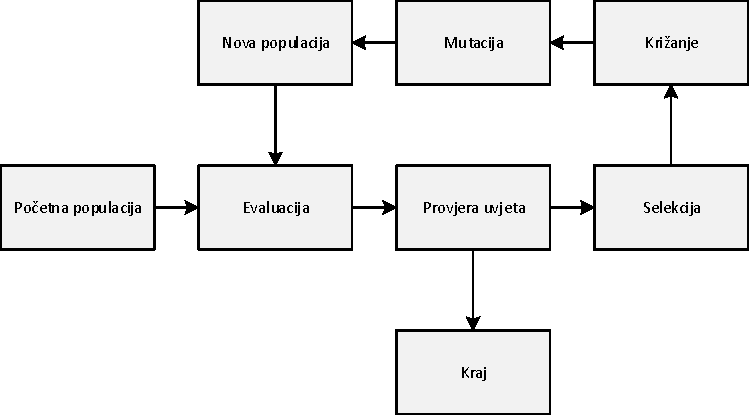
\includegraphics[width=0.7\textwidth]{Images/Gen.pdf}
    \captionsetup{justification=centering}
    \caption{Slijed rada generacijskog genetskog algoritma \cite{optjava}}
    \label{fig:gen}
\end{figure}

\subsubsection{Kromosom}
Kromosom korišten u genetskom algoritmu modelira jednu jedinku, odnosno služi kao reprezentacija jednog rješenja.
Kako se algoritam koristi u svrhu treniranja neuronske mreže, kromosom je predstavljen nizom realnih brojeva koji odgovaraju težinama ulaza neurona neuronske mreže.

\subsubsection{Evaluacija}
Prilikom evaluacije je potrebno odrediti koliko je određena jedinka uspješna, što se u ovom slučaju mjeri kao postotak uspješno klasificiranih podataka iz skupa podataka za treniranje.
Skup za treniranje sastoji se od $15910$ slika veličine $75x75$ slikovnih elemenata.
Slike su unutar skupa podijeljene na $10$ kategorija gdje svaka od njih predstavlja po jednu moguću vrijednost vrha ćelije kako je prikazano na slici \ref{fig:corners}, te kategorije u kojoj se nalaze sve one slike koje na sebi ne sadrže element tablice.
Dobrota jedinke prvotno je bila definirana samo kao postotak uspješno klasificiranih slika.
Takav pristup je imao problema uzrokovanih neproporcionalnim količinama podataka svake od kategorije (primjerice postoji $13950$ slika koje nisu elementi tablice), zbog čega je jedinka mogla imati velik postoatk uspješnosti na način da sve klasificira kao nešto što nije element tablice.
Taj je problem moguće riješiti povećanjem skupa za treniranje, što nije jednostavno izvedivo.
Drugo rješenje koje je i iskorišteno u ovom slučaju je promjena evaluacijske funkcije na način da računa postotak uspješne klasifikacije za svaku pojedinu kategoriju podataka te kao konačan rezultat koristi aritmetičku sredinu tako dobivenih postotaka.
 
\subsubsection{Selekcija}
U koraku selekcije potrebno je odabrati dvije jedinke koje će biti korištene u daljnjem postupku križanja kako bi se stvorila nova jedinka.
Postoje različiti postupci selekcija, a cilj istih je mogućnost utjecanja na to koje će jedinke stvarati potomstvo. 
Ako se uvijek biraju samo najbolje jedinke, populacija kroz samo nekoliko generacija u potpunosti gubi genetsku raznolikost zbog čega lako zapinje u lokalnim optimumima.
S druge strane, ako se sve jedinke biraju nasumično s jednakom vjerojatnošću, populacija neće napredovati te algoritam neće konvergirati ka boljim rješenjima.\\
Kako bi se ostvario balans između navedena dva načina odabira, u implementaciji su korištena $2$ načina selekcije roditelja.
Prvi roditelj se bira nasumično, gdje svaka jedinka ima jednaku vjerojatnost biti odabrana.
Drugi roditelj se bira korištenjem turnirske selekcije, koja odabire određen broj potencijalnih roditelja (u ovom slučaju je korištena veličina turnira $3$) te od tako nasumično odabranih roditelja odabire onoga sa najvećom funkcijom dobrote.

\subsubsection{Križanje}
Nakon što su odabrani roditelji provodi se križanje. 
U ovom je koraku potrebno stvoriti novu jedinku kombinacijom genetskog materijala roditelja. 
Kao i u prethodnom koraku i ovdije se javlja problem mogućnosti konvergiranja rješenja u lokalni optimum te postoje različiti pristupi kojima je moguće efikasno izvesti ovu operaciju.
U ovom radu korišteno je križanje BLX-$\alpha$ koje radi na način da svaku vrijednost određuje kao slučajnu vrijednost uniformne distribucije u intervalu vrijednosti roditelja kako je prikazano na slici \ref{fig:blx}, a što je detaljno opisano u knjizi \cite{GeneticAlgorithms}. 
Kako bi se smanjilo sažimanje populacije, interval iz kojega se bira vrijednost pojedinog elementa djeteta se proširuje za $\alpha$ posto, čime se omogućava dobivanje rješenja različitih od roditelja.

\begin{figure}[ht!]
    \centering
    \includegraphics[width=0.7\textwidth]{Images/Blx-a.pdf}
    \captionsetup{justification=centering}
    \caption{Primjer rada BLX-$\alpha$ križanja}
    \label{fig:blx}
\end{figure}

\subsubsection{Mutacija}
Prilikom mutacije je potrebno promijeniti vrijednosti kromosoma koje su dobivene križanjem roditelja kako bi se uvela nova genetska raznolikost u populaciju.
Korištena je mutacija koja uz vjerojatnost od $0.05\%$ određeni element kromosoma na način da mu doda nasumičnu vrijednost iz normalne distribucije, pomnoženu sa $0.5$. 

\subsubsection{Rezultati}
\begin{figure}[ht!]
    \centering
    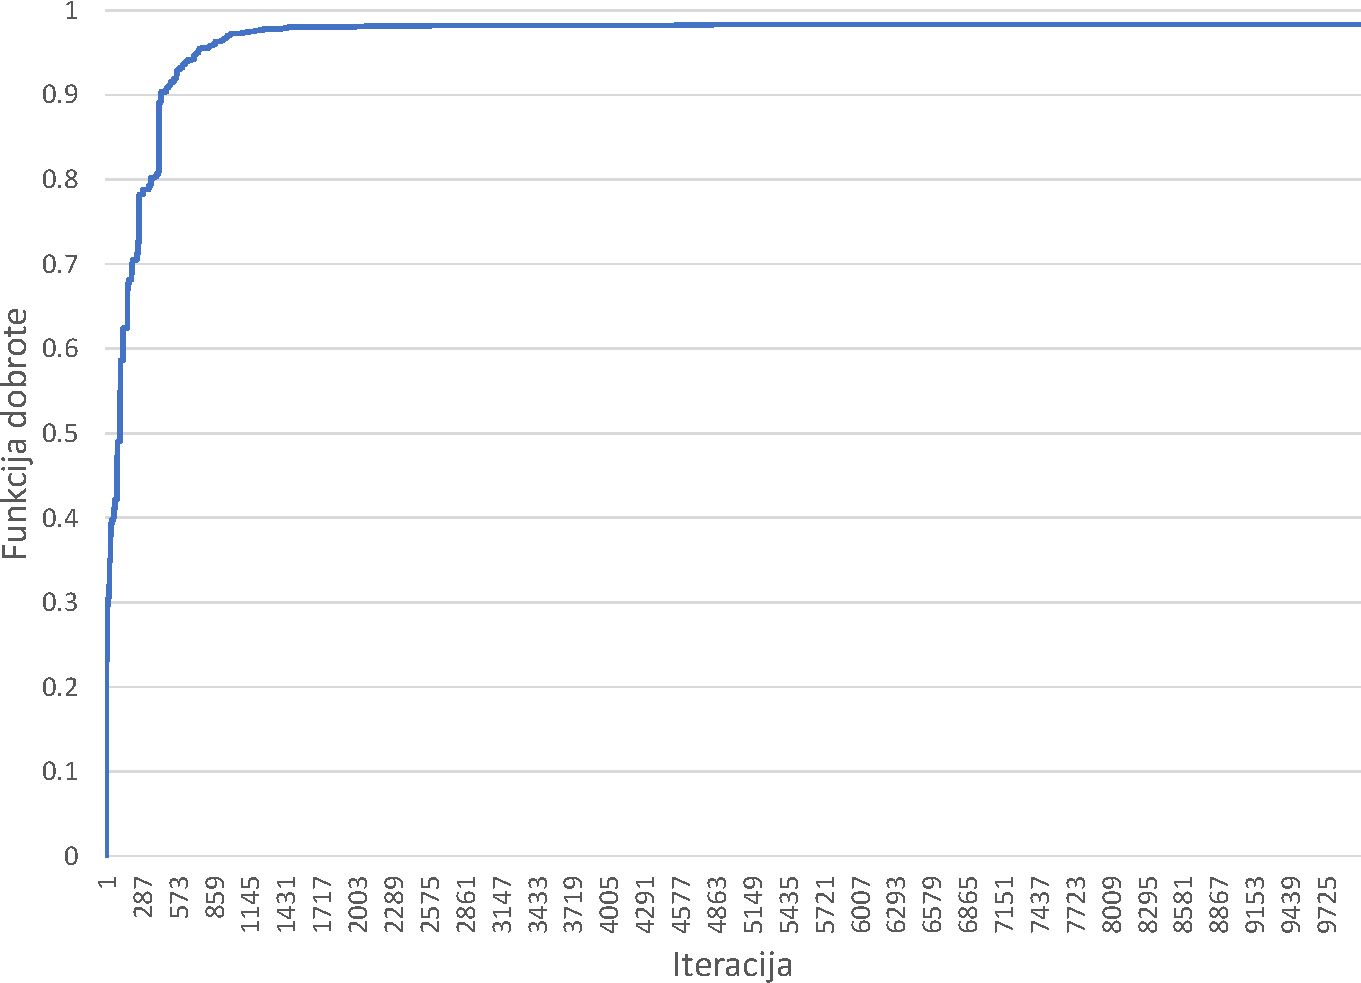
\includegraphics[width=0.85\textwidth]{Images/Ga.pdf}
    \captionsetup{justification=centering}
    \caption{Rezultati izvođenja genetskog algoritma}
    \label{fig:ga}
\end{figure}

Opisana neuronska mreža ima $500$ težina koje je potrebno postaviti, što znači da genetski algoritam radi sa kromosomima duljine $500$. 
Na slici \ref{fig:ga} prikazana je vrijednost najbolje jedinke pronađene genetskim algoritmom u odnosu na iteraciju algoritma.
Vidljivo je kako populacija na početnu brzo napreduje, no pretraga se s vremenom usporava te algoritam ne uspjeva postići zadovoljavajuće razine točnosti.

\subsection{Treniranje korištenjem backpropagation algoritma}
Drugi pristup treniranju neuronske mreže je korištenje algoritma propagacije pogreške unatrag koji je detaljno opisan u knjizi \cite{neuroracunarstvo}.
Za razliku od genetskog algoritma koji nema nikakvo znanje o tome u kojem smjeru se nalazi optimalno rješenje, ovaj algoritam računa odstupanja dobivenog rezultata od očekivanog za svaki neuron te primjenom gradijentnog spusta podešava težine kako bi smanjio pogrešku.
U ovom radu korištena je stohastička verzija navedenog algoritma koja težine ažurira na temelju greške nastale na samo jednom primjeru iz testnog skupa, a što je detaljnije objašnjeno u nastavku.


\subsubsection{Izračun pogreške}
Označimo li sa $t_o$ očekivani izlaz neuronske mreže za neuron $o$ za trenutni podatak te sa $y_o^{(k + 1)}$ stvarni izlaz neurona, greška neuronske mreže $E$ definirana je kao suma kvadratnih odstupanja, odnosno kao:
\[
    E = \frac{1}{2}\sum(t_o-y_o^{(k + 1)})^2
\]
Kako bi se ostvario gradijentni spust, potrebno je za svaku težinu izračunati gradijent za svaku težinu $w_{ij}^{(k)}$, što označava težinu koja spaja $i$-ti neuron u sloju $k$ sa $j$-tim neuronom u sloju $k+1$:
\[
    \frac{\partial E}{\partial w_{ij}^{(k)}}
\]
Tada se težina ažurira kao:
\[
    w_{ij}^{(k)} \leftarrow w_{ij}^{(k)} - \alpha \frac{\partial E}{\partial w_{ij}^{(k)}}
\]
gdje je $\alpha$ mala pozitivna konstanta poznata kao stopa učenja.

\subsubsection{Gradijent izlaznog sloja}
Potrebno je izračunati $\frac{\partial E}{\partial w_{ij}^{(k)}}$, što se može zapisati kao:
\begin{equation*}
\begin{split}
    \frac{\partial E}{\partial w_{ij}^{(k)}}
        & = \frac{\partial}{\partial w_{ij}^{(k)}} 
        \left[\frac{1}{2}\displaystyle\sum_{o = 1}^m(t_o - y_o^{(k + 1)})^2\right]\\
        & = \frac{1}{2} \displaystyle\sum_{o = 1}^m2(t_o - y_o^{(k + 1)})(-1) \frac{\partial y_o^{(k + 1)}}{\partial w_{ij}^{(k)}} \\
        & = -\displaystyle\sum_{o = 1}^m(t_o - y_o^{(k + 1)})\frac{\partial y_o^{(k + 1)}}{\partial w_{ij}^{(k)}}
\end{split}
\end{equation*}

Pritom težina $w_{ij}^{(k)}$ spaja $i$-ti neuron sloja $k$ sa $j$-tim neuronom sloja $k+1$ i nema utjecaja na ostale neurone, zbog čega su parcijalne derivacije $\frac{\partial y_o^{(k + 1)}}{\partial w_{ij}^{(k)}} = 0$ za $o != j$ pa se jednadžba može zapisati kao:

\[
    \frac{\partial E}{\partial w_{ij}^{(k)}}
    = -(t_j - y_j^{(k + 1)})\frac{\partial y_j^{(k + 1)}}{\partial w_{ij}^{(k)}}
\]
Korištenjem lančanog pravila, parcijalna derivacija iz izraza se može zapisati kao:
\[
    \frac{\partial y_j^{(k + 1)}}{\partial w_{ij}^{(k)}}
    = \frac{\partial y_j^{(k + 1)}}{\partial net_{j}^{(k+1)}}
    \frac{\partial net_{j}^{(k+1)}}{\partial w_{ij}^{(k)}}
\]
gdje je sa $net_{j}^{(k+1)}$ označena težinska suma za neuron $j$ sloja $k+1$. Kako se koriste sigmoidalna aktivacijska funkcija, vrijedi da je:
\[
    \frac{\partial y_j^{(k + 1)}}{\partial net_{j}^{(k+1)}}
    = y_j^{(k + 1)} (1 - y_j^{(k + 1)})
\]
Kako vrijedi da je
\[
    net_{j}^{(k+1)} = \displaystyle\sum_o w_{o,j}^{(k)}y_o^{(k)}    
\]
jedini član izraza koji ovisi o težini $w_{ij}^{(k)}$ je $w_{i,j}^{(k)}y_i^{(k)}$ zbog čega je parcijalna derivacija:
\[
    \frac{\partial net_{j}^{(k+1)}}{\partial w_{ij}^{(k)}} = y_i^{(k)}
\]
Uvrštavanjem dobivenog izraza u početnu jednadžbu dobiva se:
\[
    \frac{\partial E}{\partial w_{ij}^{(k)}}
    = -(t_j - y_j^{(k + 1)})
    y_j^{(k + 1)} (1 - y_j^{(k + 1)})
    y_i^{(k)}
\]
Radi jednostavnosti se greška $j$-tog neorona za dani primjer za učenje označava sa $\delta_j^{(k+1)}$ te vrijedi:
\[
    \delta_j^{(k+1)} = y_j^{(k + 1)}(1 - y_j^{(k + 1)})(t_j - y_j^{(k + 1)})
\]
Te se sada parcijalna derivacija ukupne greške može prikazati kao:
\[
    \frac{\partial E}{\partial w_{ij}^{(k)}} = -\delta_j^{(k+1)}y_i^{(k)}
\]

\subsubsection{Gradijent skrivenog sloja}
Potrebno je izračunati $\frac{\partial E}{\partial w_{ij}^{(k-1)}}$, što se može zapisati kao:
\begin{equation*}
\begin{split}
    \frac{\partial E}{\partial w_{ij}^{(k-1)}}
        & = \frac{\partial}{\partial w_{ij}^{(k-1)}} 
        \left[\frac{1}{2}\displaystyle\sum_{o = 1}^m(t_o - y_o^{(k + 1)})^2\right]\\
        & = \frac{1}{2} \displaystyle\sum_{o = 1}^m2(t_o - y_o^{(k + 1)})(-1) \frac{\partial y_o^{(k + 1)}}{\partial w_{ij}^{(k-1)}} \\
        & = -\displaystyle\sum_{o = 1}^m(t_o - y_o^{(k + 1)})\frac{\partial y_o^{(k + 1)}}{\partial w_{ij}^{(k-1)}}\\
        & = -\displaystyle\sum_{o = 1}^m(t_o - y_o^{(k + 1)})\frac{\partial y_o^{(k + 1)}}{\partial net_{o}^{(k+1)}}\frac{\partial net_o^{(k + 1)}}{\partial w_{ij}^{(k-1)}}
\end{split}
\end{equation*}
Prva parcijalna derivacija je derivacija sigmoidalne funkcije što je:
\[
    \frac{\partial y_o^{(k + 1)}}{\partial net_{o}^{(k+1)}}
    = y_o^{(k + 1)} (1 - y_o^{(k + 1)})
\]
Uvrštavanjem izračunatog u početni izraz dobiva se:
\begin{equation*}
\begin{split}
    \frac{\partial E}{\partial w_{ij}^{(k-1)}}
        & = -\displaystyle\sum_{o = 1}^m(t_o - y_o^{(k + 1)})y_o^{(k + 1)} (1 - y_o^{(k + 1)})\frac{\partial net_o^{(k + 1)}}{\partial w_{ij}^{(k-1)}}\\
        & = -\displaystyle\sum_{o = 1}^m\delta_o^{(k+1)}\frac{\partial net_o^{(k + 1)}}{\partial w_{ij}^{(k-1)}}
\end{split}
\end{equation*}
Druga parcijalna deivacija računa se pomoću $net_o^{(k + 1)}$ koji se može zapisati kao:
\[
    net_o^{(k + 1)} = \displaystyle\sum_l w_{l,o}^{(k)}y_l^{(k)}
\]
Kako je potrebno izračunati parcijalnu derivaciju za težinu $w_{ij}^{(k-1)}$ valja uočiti da ta težina utječe samo na vrijednost neurona $j$ u sloju $k$ odnosno na vrijednost $y_j^{(k)}$, zbog čega vrijedi:
\[
    \frac{\partial net_o^{(k + 1)}}{\partial w_{ij}^{(k-1)}}
    = w_{j,o}^{(k)}\frac{\partial y_j^{(k)}}{\partial w_{ij}^{(k-1)}}
\]
Parcijalna derivacija $\frac{\partial y_j^{(k)}}{\partial w_{ij}^{(k-1)}}$ rješava se na jednak način kao i u izlaznom sloju te vrijedi:
\begin{equation*}
\begin{split}
    \frac{\partial y_j^{(k)}}{\partial w_{ij}^{(k-1)}}
        & = \frac{\partial y_j^{(k)}}{\partial net_{j}^{(k)}}
            \frac{\partial net_{j}^{(k)}}{\partial w_{ij}^{(k-1)}}\\
        & = y_j^{(k)} (1 - y_j^{(k)}) y_i^{(k - 1)}
\end{split}
\end{equation*}
Uvrštavanjem u prethodnu jednakost slijedi:
\[
    \frac{\partial net_o^{(k + 1)}}{\partial w_{ij}^{(k-1)}}
        = w_{j,o}^{(k)}y_j^{(k)} (1 - y_j^{(k)}) y_i^{(k - 1)}
\]
Što vraćanjem u početnu jednakost daje:
\begin{equation*}
\begin{split}
    \frac{\partial E}{\partial w_{ij}^{(k-1)}}
        & = -\displaystyle\sum_{o = 1}^m\delta_o^{(k+1)}w_{j,o}^{(k)}y_j^{(k)} (1 - y_j^{(k)}) y_i^{(k - 1)}\\
        & = -y_i^{(k - 1)} y_j^{(k)} (1 - y_j^{(k)})\displaystyle\sum_{o = 1}^m\delta_o^{(k+1)}w_{j,o}^{(k)}
\end{split}
\end{equation*}

Ponovno se uvodi oznaka $\delta_j^{k}$ za grešku neurona, koja je definirana kao:
\[
    \delta_j^{k} = y_j^{(k)} (1 - y_j^{(k)})\displaystyle\sum_{o = 1}^m\delta_o^{(k+1)}w_{j,o}^{(k)} 
\]
Te se sada konačni rezultat može zapisati kao:
\[
    \frac{\partial E}{\partial w_{ij}^{(k-1)}} =
    -y_i^{(k - 1)}\delta_j^{k}
\]

\subsubsection{Rezultati}
\begin{figure}[ht!]
    \centering
    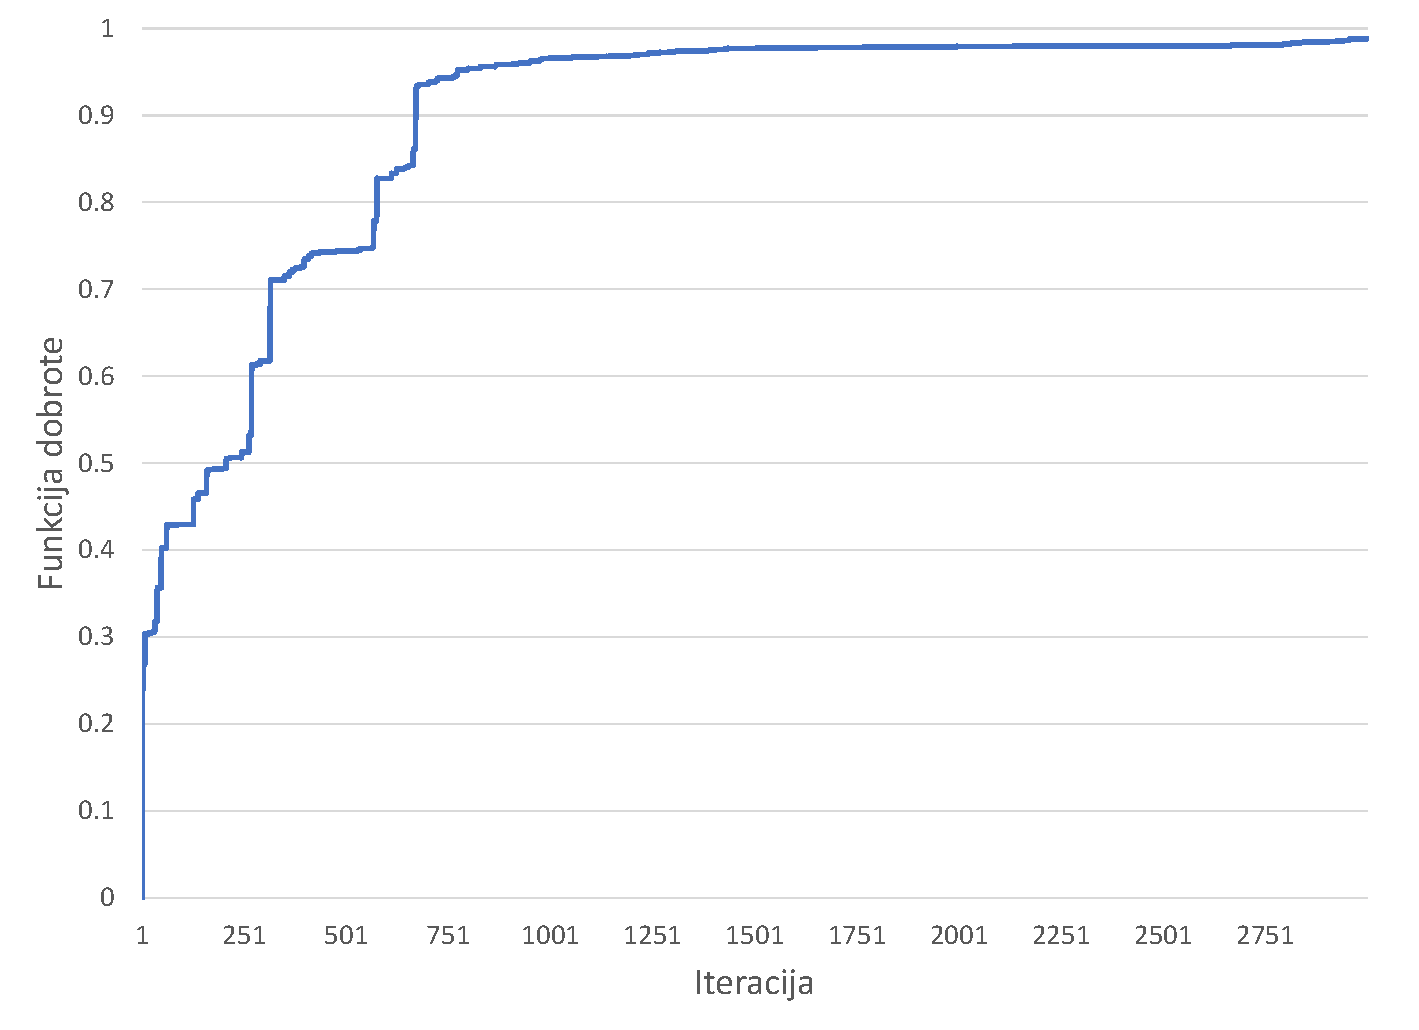
\includegraphics[width=0.85\textwidth]{Images/Backprop.pdf}
    \captionsetup{justification=centering}
    \caption{Rezultati izvođenja algoritma backpropagation}
    \label{fig:backprop}
\end{figure}

Primjena ovako opisanog algoritma stvara probleme zbog činjenice da se broj podataka za pojedine kategorije skupa za učenje drastično razlikuju.
To je riješeno na način da se prilikom ažuriranja vrijednosti težine, osim sa stopom učenja podatak množi i sa kontantom koja je obrnuto proporcionalna broju uzoraka za trenutnu kategoriju podatka.
Vidljivo je kako u početnim iteracijama algoritma postotak točne klasifikacije korištenjem algoritma backpropagation raste približno slično rastu funkcije dobrote genetskog algoritma.
Najveća razlika je uočiva kod vrijednosti koje prepoznaju više od $0.9$ podataka točno.
Kod ovog algoritma takve se neuronske mreže i dalje unaprijeđuju što je vidljivo blagim nagibom krivulje na slici \ref{fig:backprop}.
Za razliku od genetskog algoritma, ovaj algoritam uspijeva doći do vrijednosti od preko $0.99$ na testu za učenje.

\section{AdaBoost algoritam}
Za potrebe ovog klasifikacijskog algoritma potrebno je odrediti način na koji se uče slabi klasifikatori.
Svaki slabi klasifikator sastoji se od značajke, praga, konstante $p$ koja određuje vrstu nejednakosti te vrijednosti $\alpha$ koja određuje koliko je klasifikator značajan, odnosno koliko nejgov izlaz doprinosi konačnoj odluci jakog klasifikatora.
Vrijednost $\alpha$ računa se na temelju ostalih argumenata klasifikatora na skupu podataka za treniranje koji je jednak skupu podataka korištenom prilikom treniranja umjetne neuronske mreže.
Ostale parametre je potrebno odabrati na način da se minimizira pogreška klasifikatoar, što je učinjeno na način da se nasumično odabere značajka koja će se koristiti te se ona inicijalizira sa nasumično odabranim vrijednostima.
Ostali parametri također su nasumično odabrani te se za tako dobiven klasifikator računa težinska pogreška na skupu podataka za učenje.
Postupak se ponavlja velik broj puta kako bi se dobio klasifikator sa čim manjom pogreškom, koji se koristi prilikom izrade jakog klasifikatora.
\begin{figure}[ht!]
    \centering
    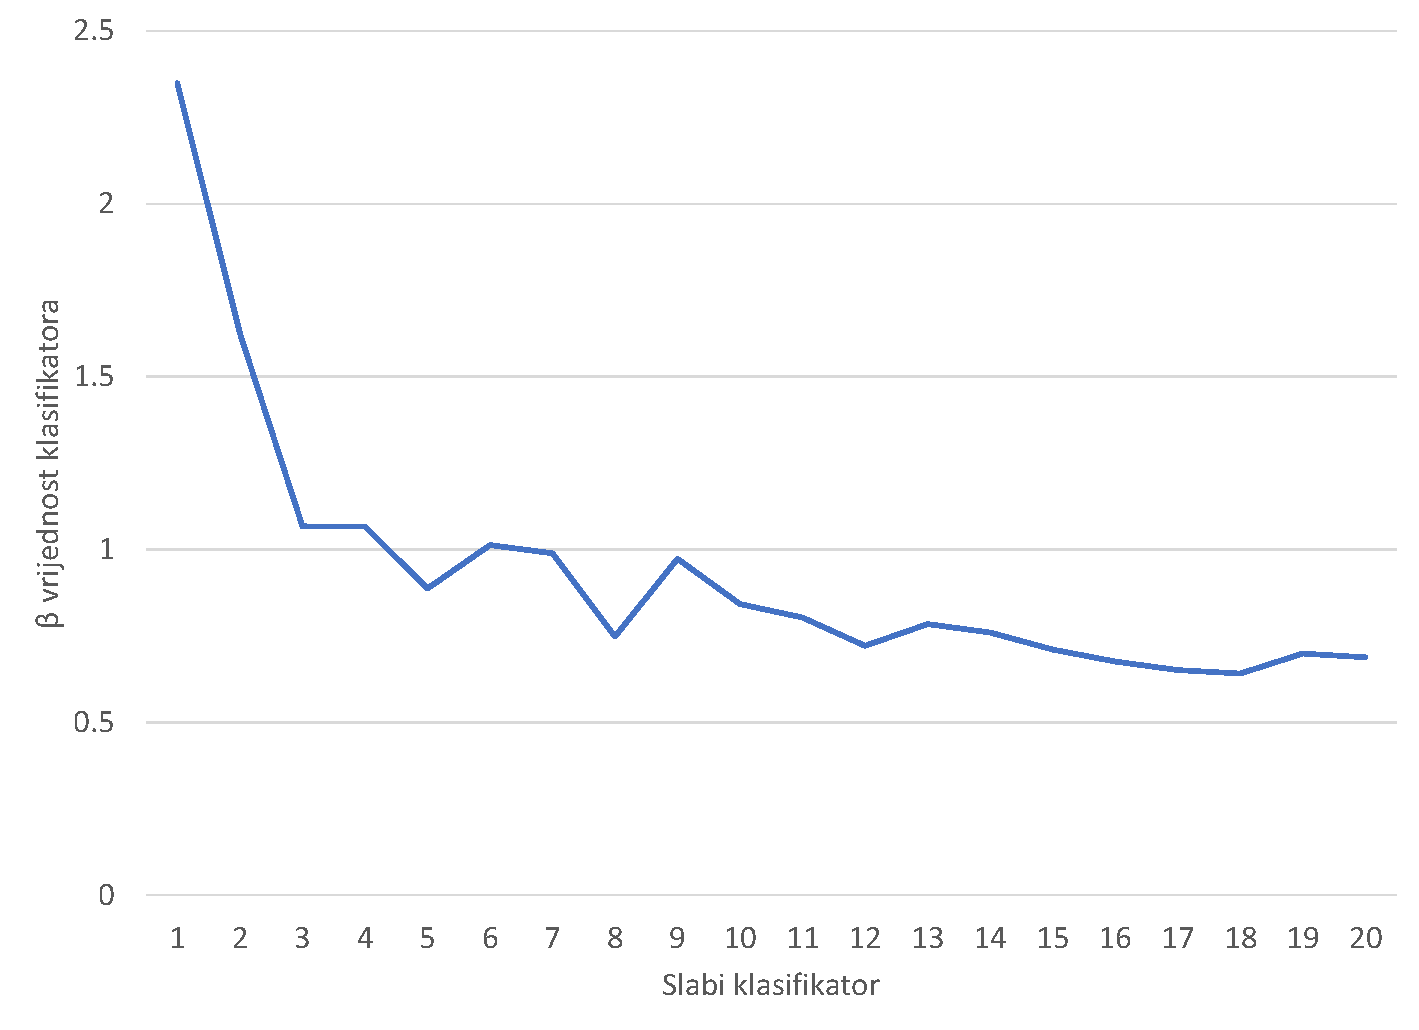
\includegraphics[width=0.85\textwidth]{Images/Ada.pdf}
    \captionsetup{justification=centering}
    \caption{$\alpha$ vrijednosti pojedinih slabih klasifikatora}
    \label{fig:ada}
\end{figure}

Graf na slici \ref{fig:ada} prikazuje $\alpha$ vrijednosti za slabe klasifikatore korištene u izradi jakog klasifikatora. 
Evidentno je kako najveću $\alpha$ vrijednost, a time i najveći doprinos u klasifikaciji ima prvi slabi klasifikator. 
Svaki sljedeći klasifikator u pravilu ima sve manju $\alpha$ vrijednost, kao što je i očekivano zbog toga što je preostale podatke sve teže i teže točno klasificirati. 
Zbog trenda pada doprinosa svakog sljedećeg klasifikatora moguće je jaki klasifikator izgraditi korištenjem prvih nekoliko slabih klasifikatora (u ovom slučaju korišteno je $20$ slabih klasifikatora), jer je sigurno da sljedeći klasifikator neće značajno doprinjeti ukupnom rezultatu, premda će usporiti pretragu.


\chapter{Zaključak}
Zaključak.


\bibliography{literatura}
\bibliographystyle{fer}

\begin{sazetak}
Sažetak na hrvatskom jeziku.

\kljucnerijeci{Ključne riječi, odvojene zarezima.}
\end{sazetak}

\engtitle{Table Extraction on Scanned Documents}
\begin{abstract}
Abstract.

\keywords{Keywords.}
\end{abstract}

\end{document}
